\chapter{Design}

\section{Overall System Design}

\subsection{Short description of the main parts of the system}

\begin{itemize}
	\item \textbf{GCSE Trigonometry and Pythagoras Education System:}
	\begin{itemize}
		\item General User Interface
		\item Getting Username and Password
		\item Navigating User's Personal Account User Interface
		\item Setting Homework From Administrator
		\item Running Individual Lessons
		\item Running Individual Homeworks
		\item Accepting User Inputs
		\item Outputting Error Exception Messages
		\item Recording Homework Results On Database
		\item Viewing Results in Database
	\end{itemize}
\end{itemize}

\begin{itemize}
	\item General User Interface
	\begin{itemize}
		\item This is the general layout of the interface across the system; the same layout pattern, same colour scheme, same positioning design.
		\item This will provide the user with the ability to navigate the parts of the system that they have access to, and enable them to select tasks, submit homeworks, and access the database to view their personal and homework records.
	\end{itemize}
\end{itemize}

\begin{itemize}
	\item Getting Username and Password
	\begin{itemize}
		\item This will come in the very first window every time the user or administrator wants to access the program; it will ask them to log in so that they can view their own personal account, with all of their homework progress and personal records.
		\item It will mainly consist of two text boxes in the centre of the screen, one prompting a username and the other a password underneath. 
		\item If invalid information is input it will display an error message asking the user to retry. There will be no limit to the number of attempts a user can have; it won't lock them out of their computer if they keep getting it wrong.
	\end{itemize}
\end{itemize}

\begin{itemize}
	\item Navigating User's Personal Account User Interface
	\begin{itemize}
		\item This is essentially the functionality between each window. The user will have a range of buttons to press which will then open the relevant window, and then will have the option to return, making each part of the system accessible.
	\end{itemize}
\end{itemize}

\begin{itemize}
	\item Setting Homework From Administrator
	\begin{itemize}
		\item The function which makes the user aware of which homework has been set; the administrator will set it, the system will acknowledge it, and then notify the required users to do it.
		\item The reverse will work similarly; the user will complete the homework and the administrator will be notified. They will also be notified if the user hasn't completed it before the due date.
	\end{itemize}
\end{itemize}

\begin{itemize}
	\item Running Individual Lessons
	\begin{itemize}
		\item The module that runs for each lesson. Each lesson will have its own set of windows, containing the inputs, outputs and graphics to accurately represent what is being taught e.g Pythagoras Theorem.
		\item These will only be opened, navigated and closed as nothing from these is recorded in the database; they are effectively read only.
	\end{itemize}
\end{itemize}

\begin{itemize}
	\item Running Individual Homeworks
	\begin{itemize}
		\item The module that runs for each homework, saved so that each different homework task is always the same, in order to avoid confusion. 
		\item When the homework is run, inputs are accepted, outputs are given, and at the end the appropriate information is recorded in the database.
	\end{itemize}
\end{itemize}

\begin{itemize}
	\item Accepting User Inputs
	\begin{itemize}
		\item Each input type in the system, be it the general user interface, a lesson or a homework, will be accepted.
		\item Once accepted, it will be validated, and if invalid, the appropriate error message will be displayed.
		\item Different types of inputs are:
		\begin{itemize}
			\item Text Boxes
			\item Drag and Drop Images
			\item Image Modification
			\item Buttons 
		\end{itemize} 
		\item If valid, the system will either allow them access to their account, or add a mark to their homework task score.
	\end{itemize}
\end{itemize}

\begin{itemize}
	\item Outputting Error Exception Messages
	\begin{itemize}
		\item If a user's input is invalid, the appropriate error message will be displayed.
		\item Each error message will appear for 5 seconds and then disappear automatically.
		\item These are the variations of error messages and their causes:
		\begin{itemize}
			\item Invalid Username
			\item Invalid Password
			\item Invalid Data Type
			\item Wrong Answer 1{$^s$}{$^t$}
			\item Wrong Answer 2{$^n$}{$^d$}
			\item Unauthorised Access
		\end{itemize}
	\end{itemize}
\end{itemize}

\begin{itemize}
	\item Recording Homework Results On Database
	\begin{itemize}
		\item Every time a user completes a homework, the results will be recorded in the database, including the \textbf{OverallPercentScore}, \textbf{IndividualPercentScore(s)}, and \textbf{Rating}. 
		\item The user will be able to view their results in their personal database section, and the administrator will be able to view these results in the entire class database for that task.
	\end{itemize}
\end{itemize}

\begin{itemize}
	\item Viewing Results in Database
	\begin{itemize}
		\item A student will be able to click a button on the home screen to take them to the database view, where they will clearly see all of their personal results
		\item A teacher will be able to click a button on the home screen to take them to the database view, where they will clearly see all of the students results in any of their own classes, and they will be able to scroll through each student in alphabetical order on a scroll bar on the side to find individual's results
		\item An administrator (teacher) can amend a database value if it is necessary, although it is unlikely that it will be
		\item A return button will take them straight back to the home page to continue using the system
	\end{itemize}
\end{itemize}

\subsection{System flowcharts showing an overview of the complete system}

\textbf{This flowchart represents the system accessible for a student/user: }

%U:/git/COMP4Coursework2/Design/
%C:/Users/Jordan/git/COMP4Coursework2/Design

\begin{figure}[H]
    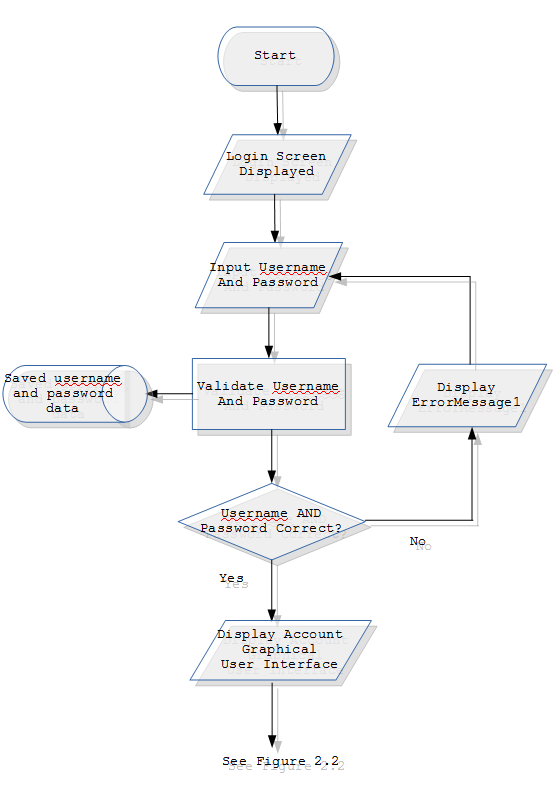
\includegraphics[width=\textwidth]{U:/git/COMP4Coursework2/Design/user_flow_1}
    \label{fig:print_function_result}\caption{}
\end{figure}

\begin{figure}[H]
    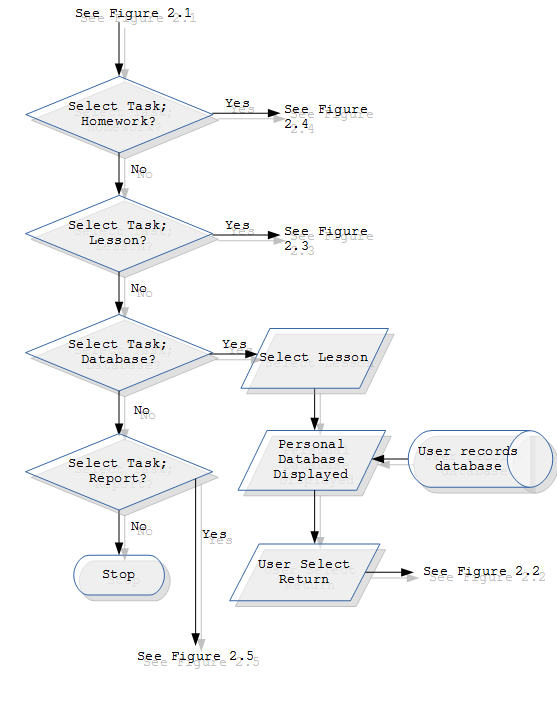
\includegraphics[width=\textwidth]{U:/git/COMP4Coursework2/Design/user_flow_2}
    \label{fig:print_function_result}\caption{}
\end{figure}

\begin{figure}[H]
    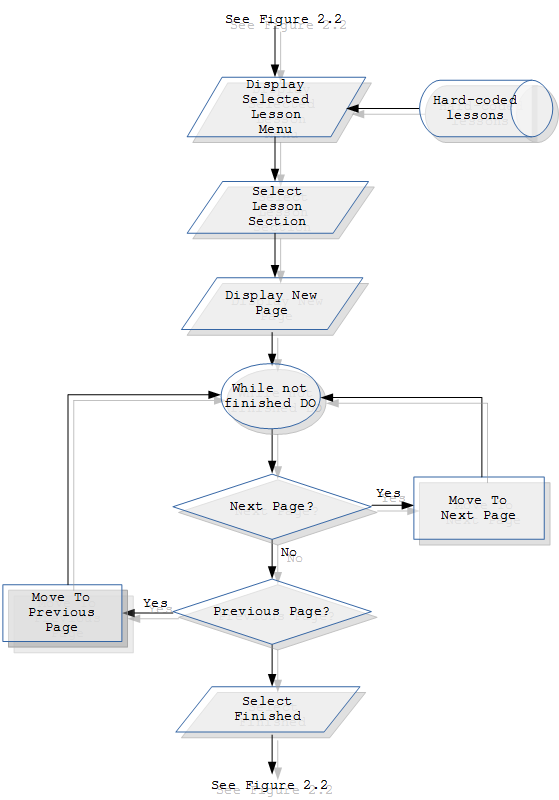
\includegraphics[width=\textwidth]{U:/git/COMP4Coursework2/Design/user_flow_3}
    \label{fig:print_function_result}\caption{}
\end{figure}

\begin{figure}[H]
    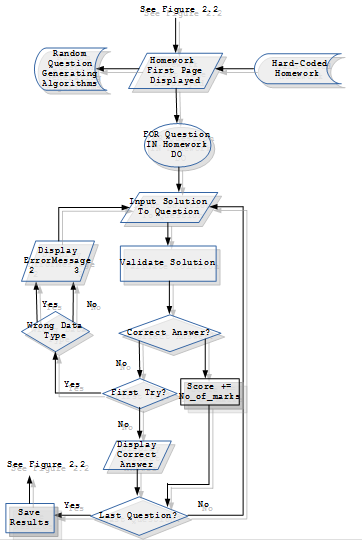
\includegraphics[width=\textwidth]{U:/git/COMP4Coursework2/Design/user_flow_4}
    \label{fig:print_function_result}\caption{}
\end{figure}

\textbf{This flowchart represents the system accessible for a teacher/administrator: }

\begin{figure}[H]
    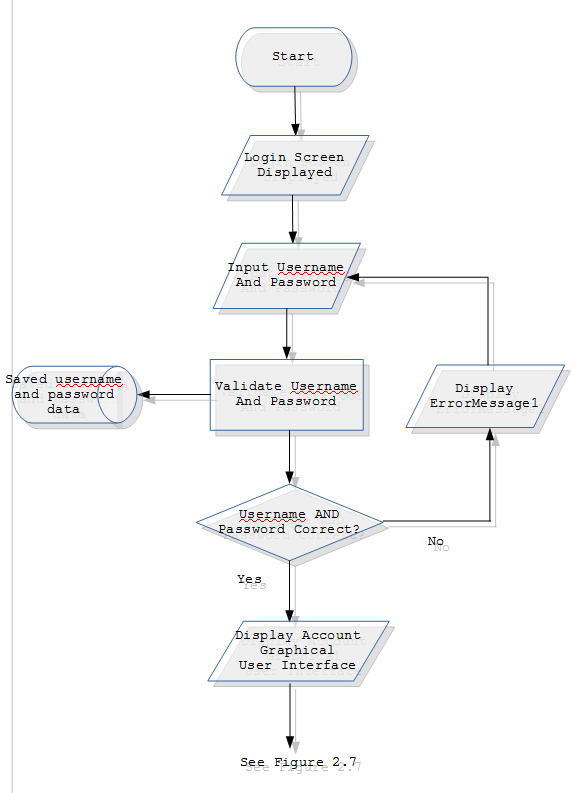
\includegraphics[width=\textwidth]{U:/git/COMP4Coursework2/Design/admin_flow_1}
    \label{fig:print_function_result}\caption{}
\end{figure}

\begin{figure}[H]
    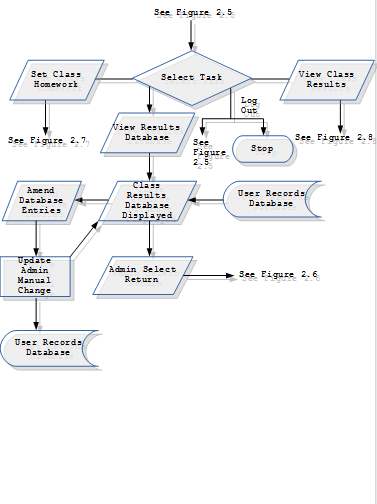
\includegraphics[width=\textwidth]{U:/git/COMP4Coursework2/Design/admin_flow_2}
    \label{fig:print_function_result}\caption{}
\end{figure}

\begin{figure}[H]
    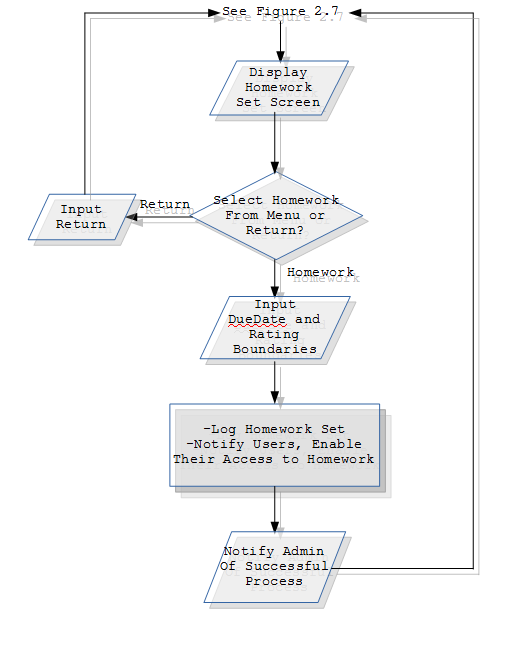
\includegraphics[width=\textwidth]{U:/git/COMP4Coursework2/Design/admin_flow_3}
    \label{fig:print_function_result}\caption{}
\end{figure}

\begin{figure}[H]
    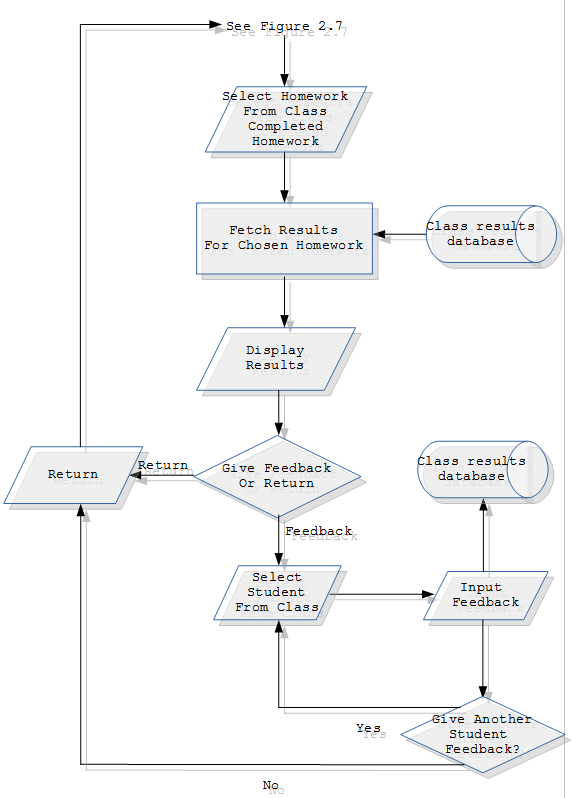
\includegraphics[width=\textwidth]{U:/git/COMP4Coursework2/Design/admin_flow_4}
    \label{fig:print_function_result}\caption{}
\end{figure}

\section{User Interface Designs}

%U:/git/COMP4Coursework2/Design
%U:/git/COMP4Coursework2/Design/

\begin{figure}[H]
    \label{fig:print_function_result}\caption{Login Screen}
    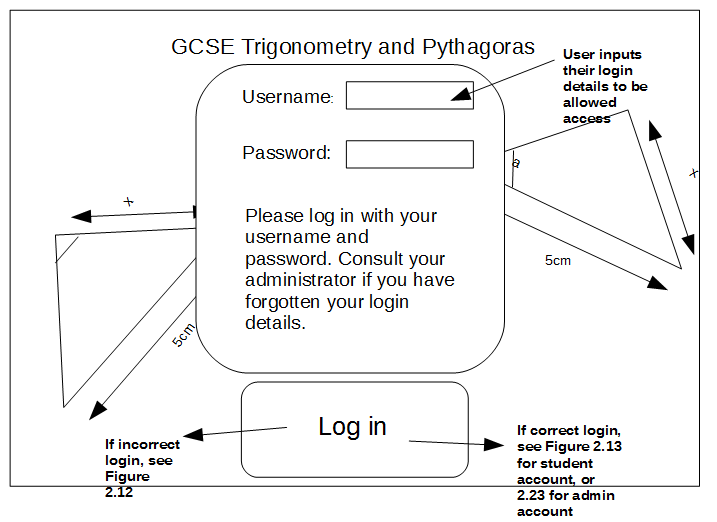
\includegraphics[width=\textwidth]{U:/git/COMP4Coursework2/Design/figure_2_9}
\end{figure}

\begin{figure}[H]
    \label{fig:print_function_result}\caption{ErrorMessage2}
    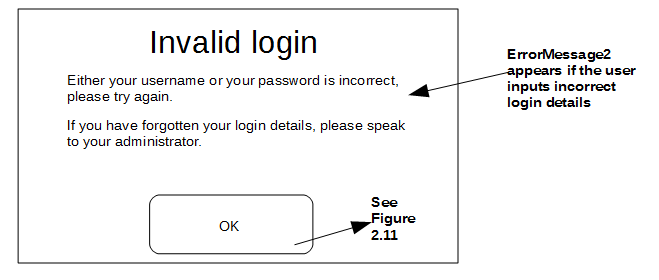
\includegraphics[width=\textwidth]{U:/git/COMP4Coursework2/Design/figure_2_10}
\end{figure}

\begin{figure}[H]
    \label{fig:print_function_result}\caption{Student Home Screen}
    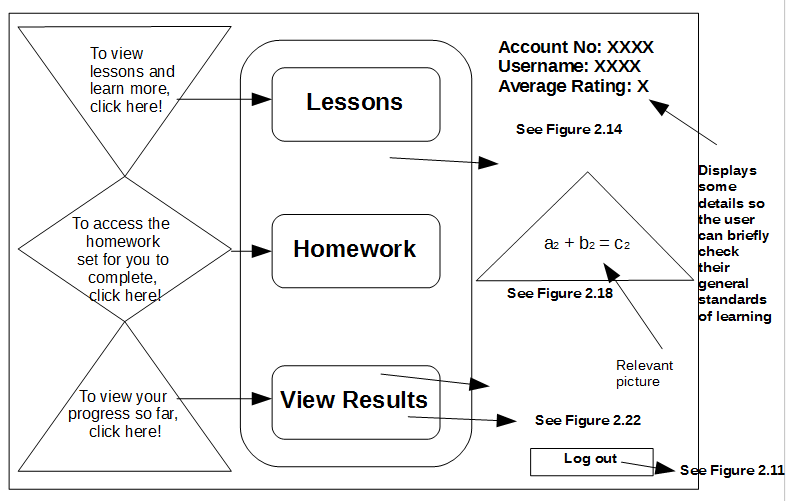
\includegraphics[width=\textwidth]{U:/git/COMP4Coursework2/Design/figure_2_11}
\end{figure}

\begin{figure}[H]
    \label{fig:print_function_result}\caption{Lesson Topic Menu}
    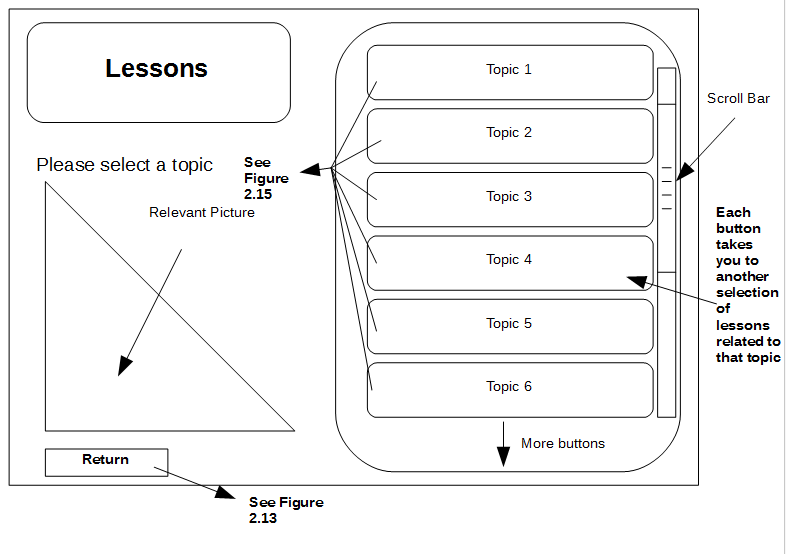
\includegraphics[width=\textwidth]{U:/git/COMP4Coursework2/Design/figure_2_12}
\end{figure}

\begin{figure}[H]
    \label{fig:print_function_result}\caption{Lesson Menu}
    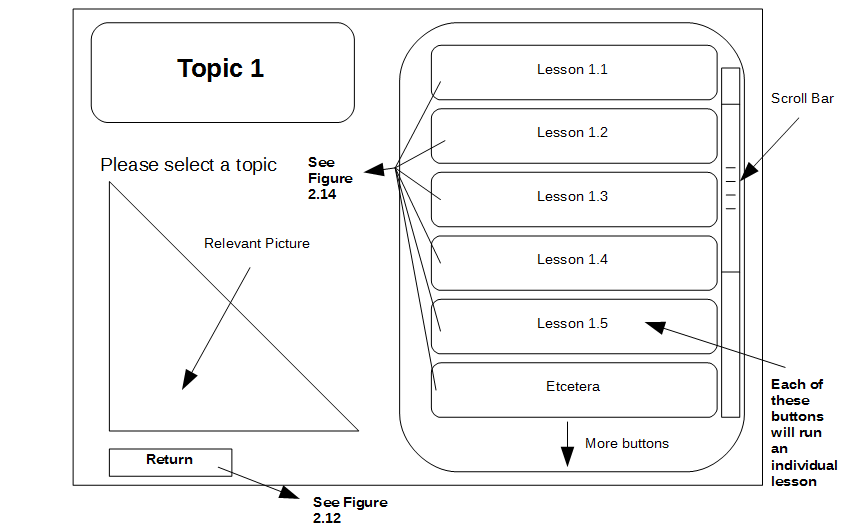
\includegraphics[width=\textwidth]{U:/git/COMP4Coursework2/Design/figure_2_13}
\end{figure}

\begin{figure}[H]
    \label{fig:print_function_result}\caption{First Lesson Screen}
    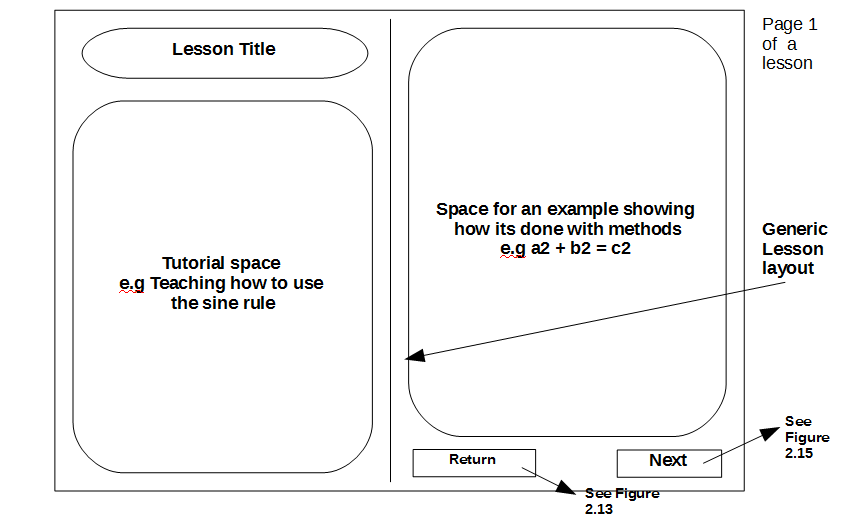
\includegraphics[width=\textwidth]{U:/git/COMP4Coursework2/Design/figure_2_14}
\end{figure}

\begin{figure}[H]
    \label{fig:print_function_result}\caption{Second Lesson Screen}
    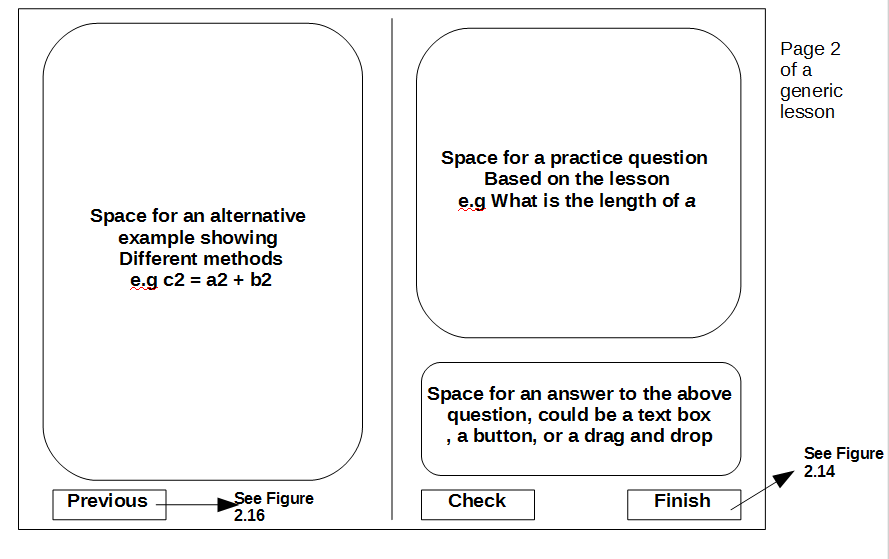
\includegraphics[width=\textwidth]{U:/git/COMP4Coursework2/Design/figure_2_15}
\end{figure}

\begin{figure}[H]
    \label{fig:print_function_result}\caption{Homework Topic Menu}
    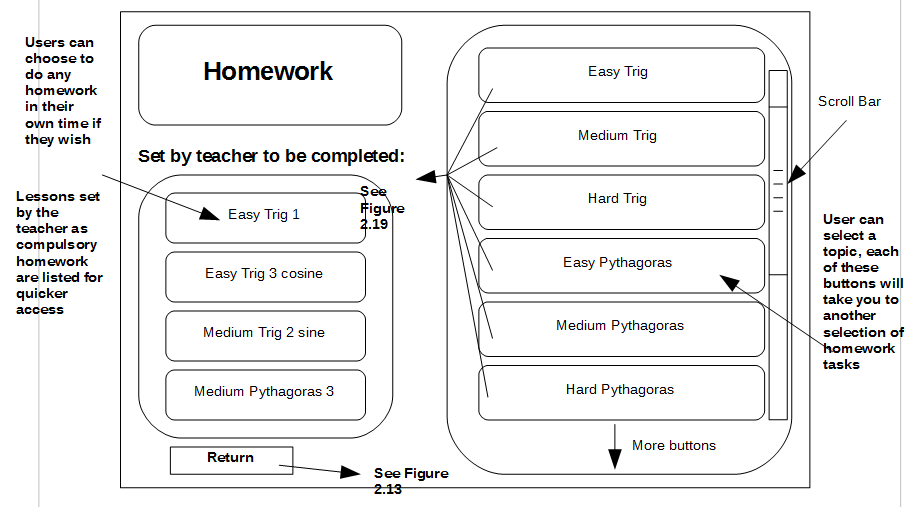
\includegraphics[width=\textwidth]{U:/git/COMP4Coursework2/Design/figure_2_16}
\end{figure}

\begin{figure}[H]
    \label{fig:print_function_result}\caption{Homework Menu}
    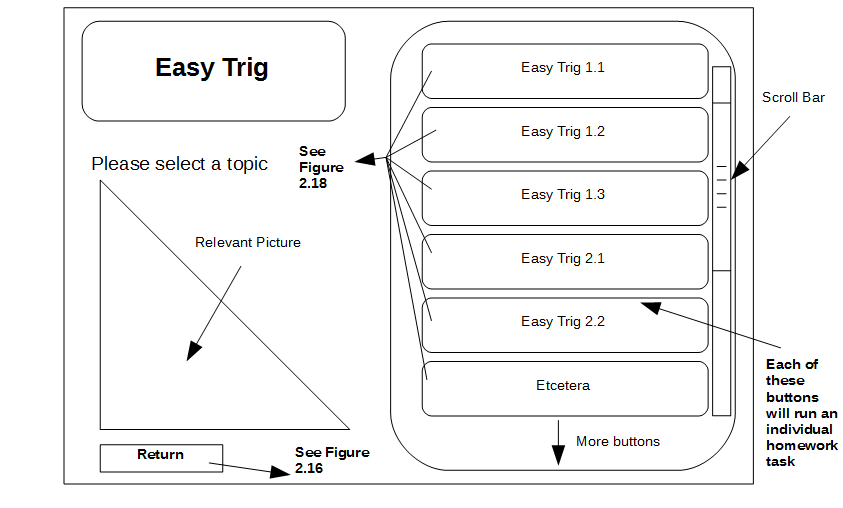
\includegraphics[width=\textwidth]{U:/git/COMP4Coursework2/Design/figure_2_17}
\end{figure}

\begin{figure}[H]
    \label{fig:print_function_result}\caption{First Homework Screen}
    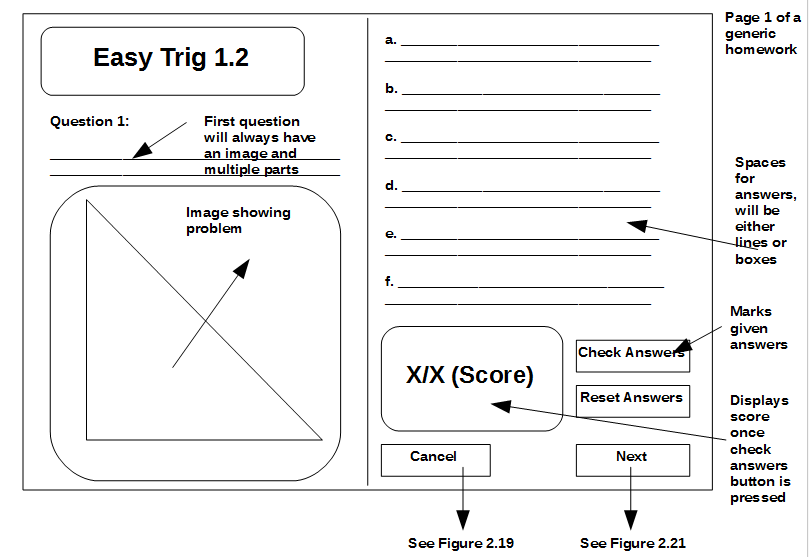
\includegraphics[width=\textwidth]{U:/git/COMP4Coursework2/Design/figure_2_18}
\end{figure}

\begin{figure}[H]
    \label{fig:print_function_result}\caption{Second Homework Screen}
    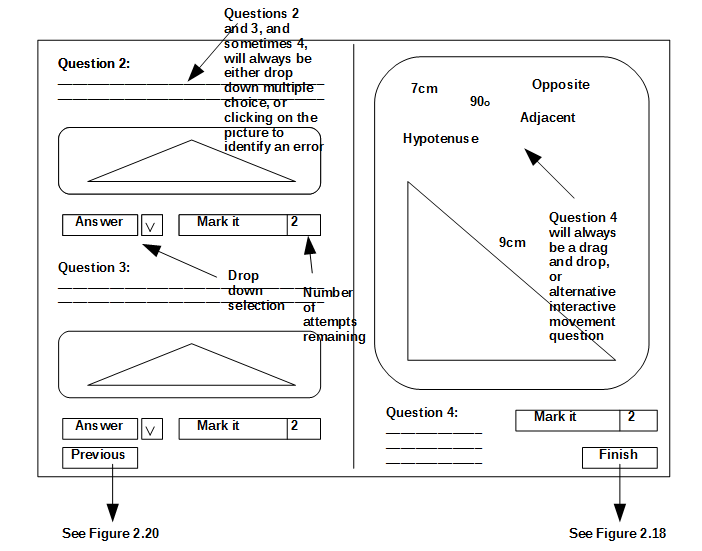
\includegraphics[width=\textwidth]{U:/git/COMP4Coursework2/Design/figure_2_19}
\end{figure}

\begin{figure}[H]
    \label{fig:print_function_result}\caption{Individual User Progress Database}
    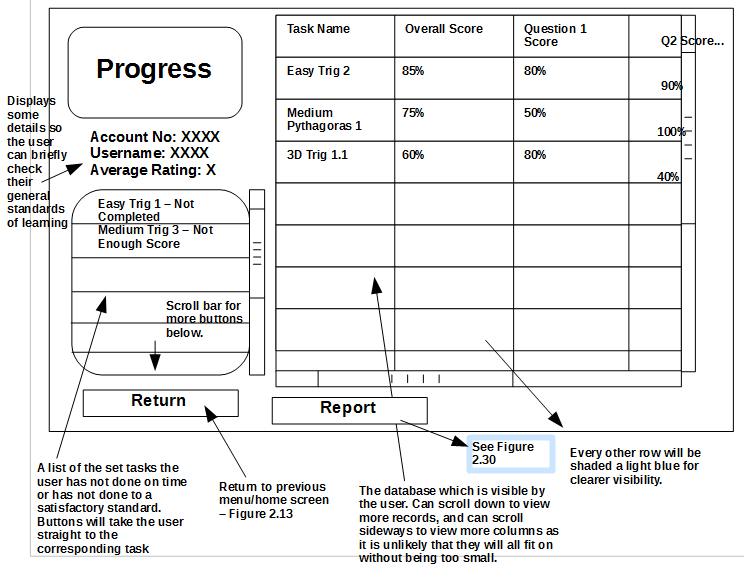
\includegraphics[width=\textwidth]{U:/git/COMP4Coursework2/Design/figure_2_20}
\end{figure}

\begin{figure}[H]
    \label{fig:print_function_result}\caption{Administrator Account Home}
    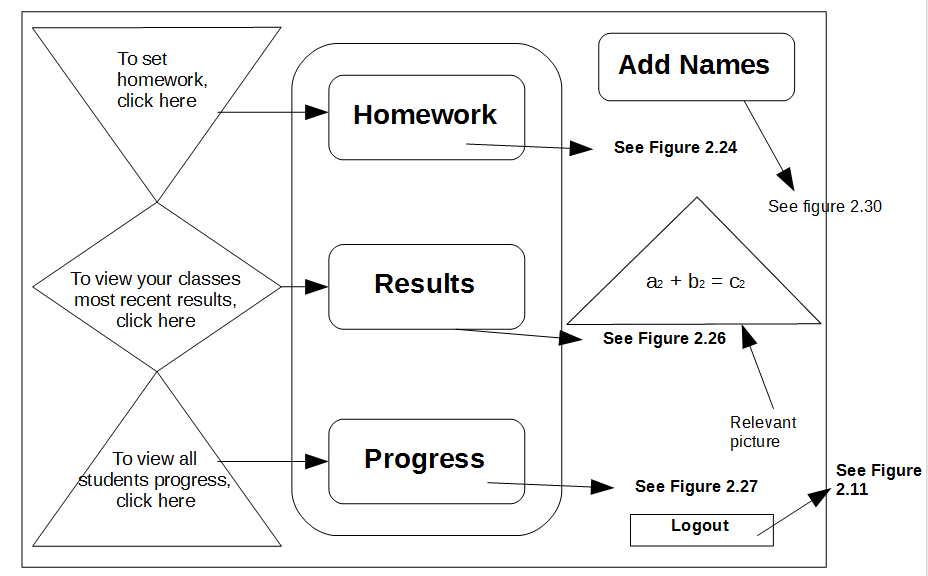
\includegraphics[width=\textwidth]{U:/git/COMP4Coursework2/Design/figure_2_21}
\end{figure}

\begin{figure}[H]
    \label{fig:print_function_result}\caption{Homework Setting Topic Menu}
    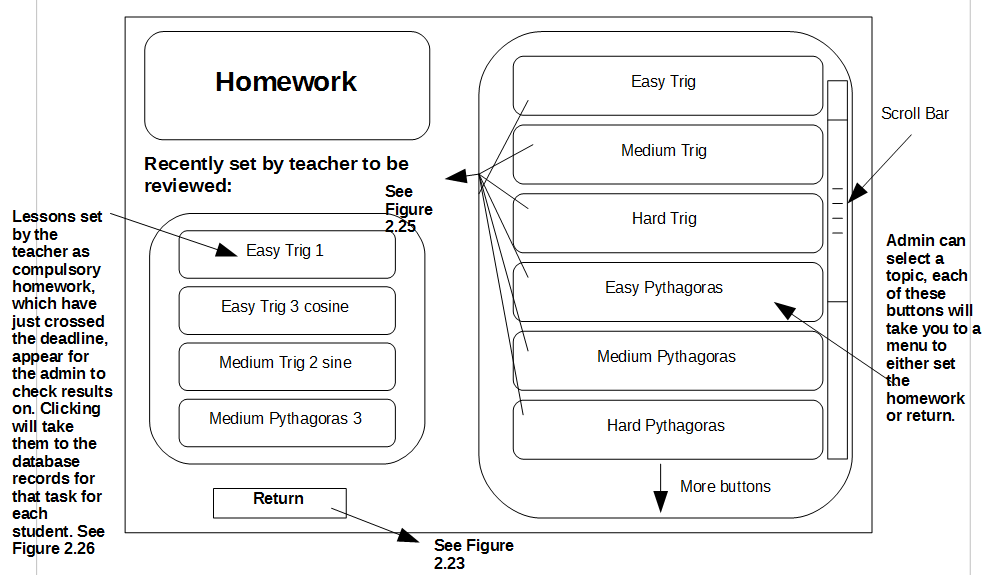
\includegraphics[width=\textwidth]{U:/git/COMP4Coursework2/Design/figure_2_22}
\end{figure}

\begin{figure}[H]
    \label{fig:print_function_result}\caption{Homework Set Screen}
    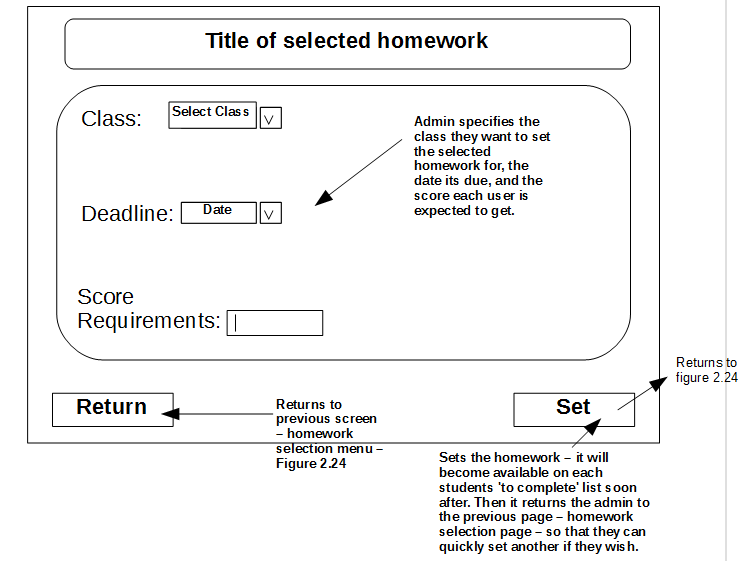
\includegraphics[width=\textwidth]{U:/git/COMP4Coursework2/Design/figure_2_23}
\end{figure}

\begin{figure}[H]
    \label{fig:print_function_result}\caption{Results Menu}
    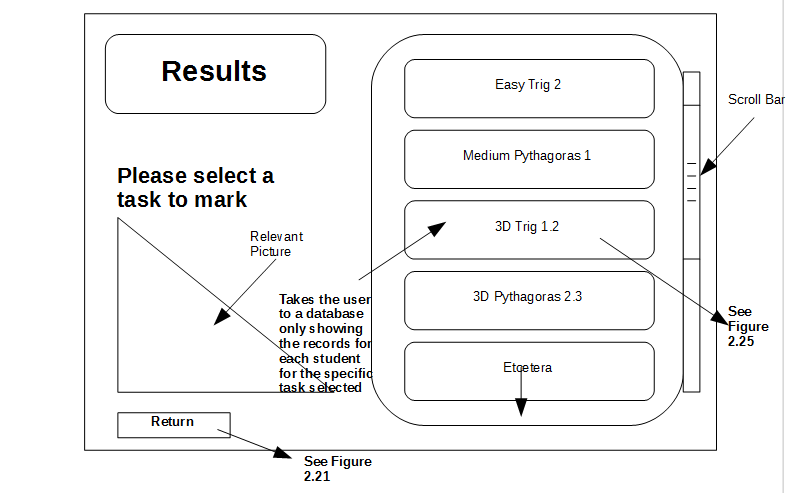
\includegraphics[width=\textwidth]{U:/git/COMP4Coursework2/Design/figure_2_24}
\end{figure}

\begin{figure}[H]
    \label{fig:print_function_result}\caption{Class Results Database}
    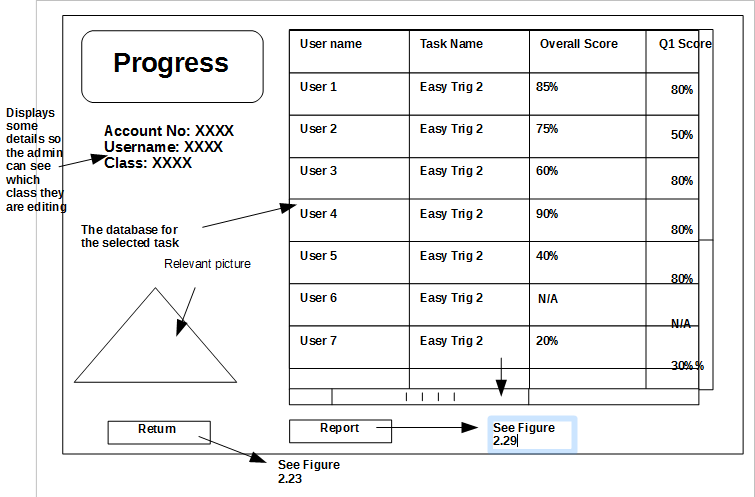
\includegraphics[width=\textwidth]{U:/git/COMP4Coursework2/Design/figure_2_25}
\end{figure}

\begin{figure}[H]
    \label{fig:print_function_result}\caption{ErrorMessage3}
    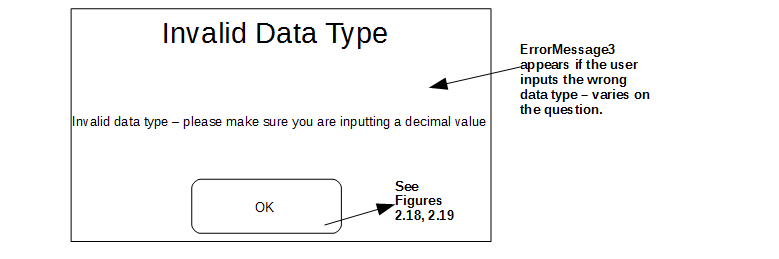
\includegraphics[width=\textwidth]{U:/git/COMP4Coursework2/Design/figure_2_26}
\end{figure}

\begin{figure}[H]
    \label{fig:print_function_result}\caption{ErrorMessage3}
    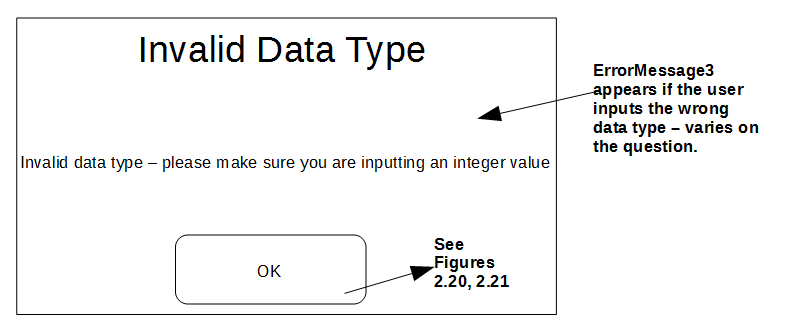
\includegraphics[width=\textwidth]{U:/git/COMP4Coursework2/Design/figure_2_27}
\end{figure}

\begin{figure}[H]
    \label{fig:print_function_result}\caption{ErrorMessage3}
    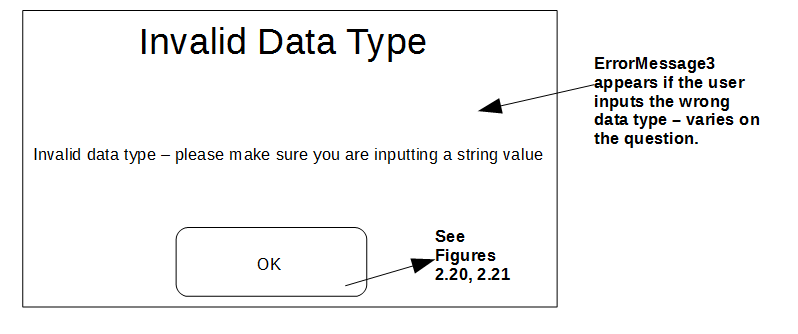
\includegraphics[width=\textwidth]{U:/git/COMP4Coursework2/Design/figure_2_28}
\end{figure}

\begin{figure}[H]
    \label{fig:print_function_result}\caption{ErrorMessage4}
    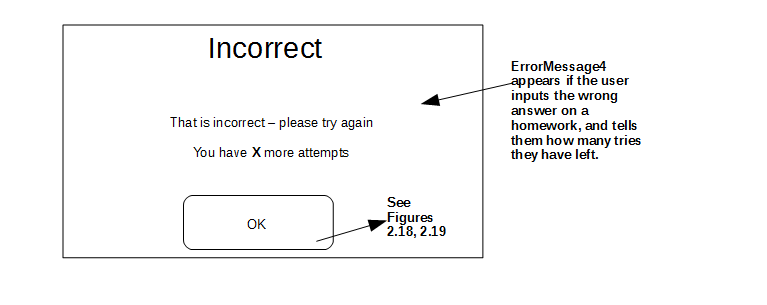
\includegraphics[width=\textwidth]{U:/git/COMP4Coursework2/Design/figure_2_29}
\end{figure}

\section{Hardware Specification}

This system will need to run on a standard desktop computer, as generally found in schools, using the Windows 7 operating system. It will need to have a screen resolution of 1920 x 1080, a 32 bit true colour scheme, a 16:9 aspect ratio, and an Intel HD Graphics 2500 card or better, running at 60p Hz. Windows 7 is required as it is still currently the operating system used by more or less every education facility, and the client will be working at such a facility. The 32 bit true colour scheme is usually the default set by the administrators, and they need a 16:9 aspect ratio, as I need to be able to make the windows fit properly on every machine at the facility, and the screens will not be resizable. The 1920 x 1080 resolution is desirable but not entirely necessary; it is achievable and will maintain the quality of the appearance of the program. The Intel HD Graphics 2500 is standard and should be able to run the system. A keyboard will be required for inputting text answers into boxes throughout the lessons, homework, and for logging in; any standard keyboard will be usable for this. Similarly, any standard mouse will be needed for navigating the GUI, clicking buttons, scrolling, using frop down boxes and dragging and dropping. A standard display will be used for the output of the system; just visual, no audio. The data for each user will be stored on a local server so that every user or administrator can view their own/all data from any of the machines at the facility. All of these requirements are able to be met by the client, who has it all available.

\section{Program Structure}

\subsection{Top-down design structure charts}

\begin{figure}[H]
    \label{fig:print_function_result}\caption{}
    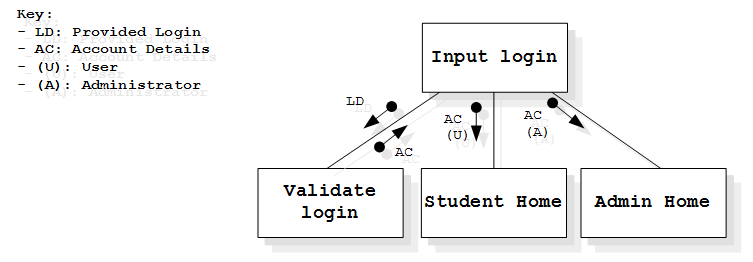
\includegraphics[width=\textwidth]{U:/git/COMP4Coursework2/Design/figure_2_30}
\end{figure}

\begin{figure}[H]
    \label{fig:print_function_result}\caption{}
    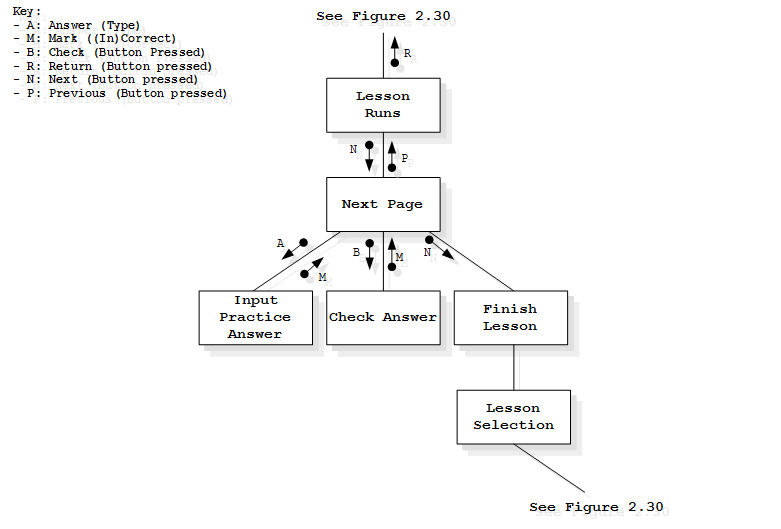
\includegraphics[width=\textwidth]{U:/git/COMP4Coursework2/Design/figure_2_31}
\end{figure}

\begin{figure}[H]
    \label{fig:print_function_result}\caption{}
    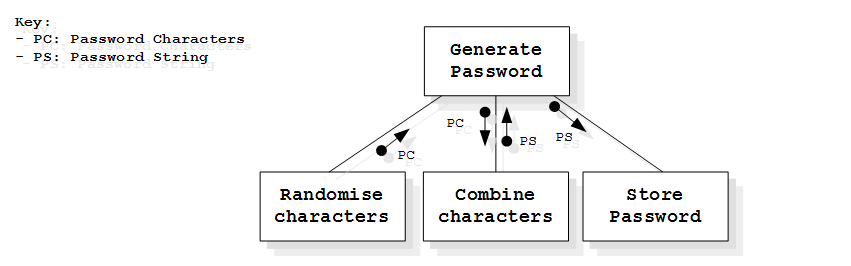
\includegraphics[width=\textwidth]{U:/git/COMP4Coursework2/Design/figure_2_32}
\end{figure}

\begin{figure}[H]
    \label{fig:print_function_result}\caption{}
    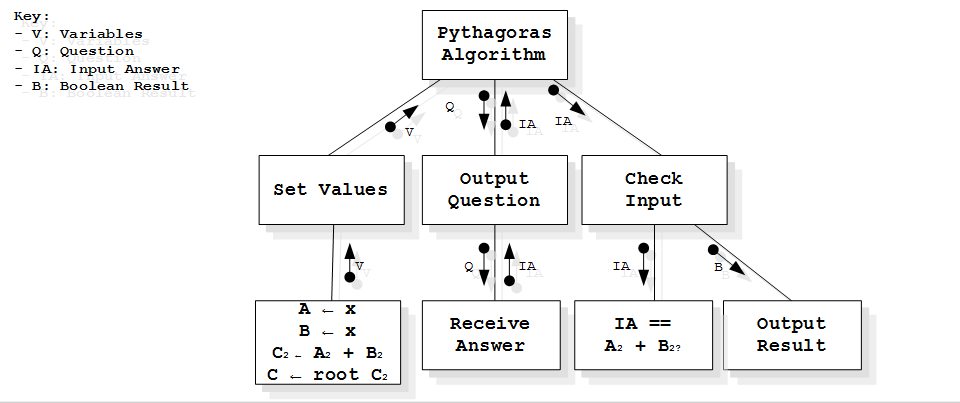
\includegraphics[width=\textwidth]{U:/git/COMP4Coursework2/Design/figure_2_33}
\end{figure}

\begin{figure}[H]
    \label{fig:print_function_result}\caption{}
    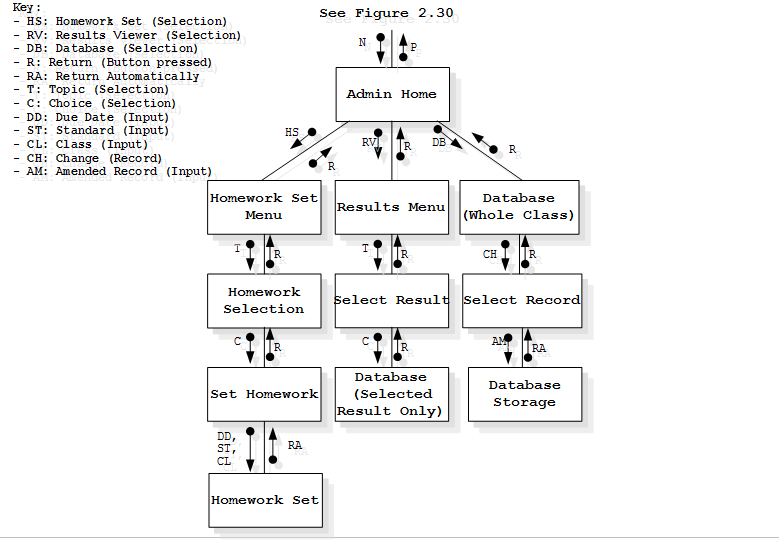
\includegraphics[width=\textwidth]{U:/git/COMP4Coursework2/Design/figure_2_34}
\end{figure}

\subsection{Algorithms in pseudo-code for each data transformation process}

\textbf{Validates the username and password when the user tries to log in:}

\begin{algorithm}[H]
\caption{Takes the logins from the database and adds them to a list from which they can be validated.}
\begin{algorithmic}[1]
\SET{$with \ open("logins.txt", mode = "r") as \ logins$}
\For{$name$}{$logins$}
	\SET{$list\_.append(name)$}
\EndFor
\RECEIVE{"Please enter your username"}
\SET{$return \ username$}
\RECEIVE{"Please enter your password"}
\SET{$return \ password$}
\SET{$count$}{$0$}
\SET{$found$}{$False$}
\While{$found = False$}{$and \ count < len(list\_)$}
	\If{$list\_[count] = str(username) \ and \ list\_[count + 2] = str(password)$}
		\SEND("Accepted")
		\SET{$found$}{$True$}
		\SET{$return \ found$}
	\Else{}
		\SEND{"Not accepted"}
		\SET{$call \ Validation$}
	\SET{$count \ += \ 1$}
	\EndIf
\EndWhile
\end{algorithmic}
\end{algorithm}

\begin{algorithm}[H]
\caption{Checks if the user's solution for the {$a^2 + b^2 = c^2$} is correct.}
\begin{algorithmic}[1]
\SET{$total\_marks$}{$0$}
\SET{$side\_a$}{$x$}
\SET{$side\_b$}{$x$}
\SET{$side\_c$}{$\sqrt{side\_a^2 + side\_b^2}$}
\SEND{$"Here \ is \ a \ right \ angled \ triangle. \ The \ length \ of \ side \ a \ is \ x$}
\SET{$centimetres, \ and \ the \ length \ of \ side \ b \ is \ x \ centimetres.$}
\SET{$Please \ calculate \ the \ length \ of \ side \ c"$}
\RECEIVE{$length$}{$"Please \ input \ the \ length \ of \ side \ c: "$}
\If {$length = side\_c$}
	\SEND{"+ 1 \ mark"}
	\SET{$total\_marks \ += \ x$}
\Else{}
	\SEND{"The \ answer \ is \ x"}
\EndIf
\end{algorithmic}
\end{algorithm}

\textbf{Alternative algorithm:}

\begin{algorithm}[H]
\caption{Same question and solution with a differently arranged formula.}
\begin{algorithmic}[1]
\SET{$total\_marks$}{$0$}
\SET{$side\_a$}{$x$}
\SET{$side\_b$}{$x$}
\SET{$side\_c^2$}{$side\_a^2 + side\_b^2$}
\SET{$side\_c$}{$\sqrt{side\_c^2}$}
\SEND{$"Here \ is \ a \ right \ angled \ triangle. \ The \ length \ of \ side \ a \ is \ x$}
\SET{$centimetres, \ and \ the \ length \ of \ side \ b \ is \ x \ centimetres.$}
\SET{$Please \ calculate \ the \ length \ of \ side \ c"$}
\RECEIVE{$length$}{$"Please \ input \ the \ length \ of \ side \ c: "$}
\If{$length = side\_c$}
	\SEND{"+ x \ marks"}
	\SET{$total\_marks \ += \ x$}
\Else{}
	\SEND{"The \ answer \ is \ x"}
\EndIf
\end{algorithmic}
\end{algorithm}

\textbf{3D Pythagoras algorithm:}

\begin{algorithm}[H]
\caption{Similar algorithm, but continues to check the user's solution for a 3D pythagoras problem.}
\begin{algorithmic}[1]
\SET{$total\_marks$}{$0$}
\SET{$left\_side\_a$}{$x$}
\SET{$middle\_side\_a$}{$x$}
\SET{$right\_side\_a$}{$x$}
\SET{$inside\_side\_a$}{$\sqrt{left\_side\_a^2 + middle\_side\_a^2}$}
\SET{$inside\_side\_b$}{$\sqrt{right\_side\_a^2 + inside\_side\_a^2}$}
\SEND{$"A \ magician \ stores \ his \ wand \ in \ a \ box.$}
\SET{$The \ box \ is \ xcm \ by \ xcm \ by \ xcm.$}
\SET{$The \ wand \ only \ just \ fits \ in \ wedged \ against \ opposite \ corners."$}
\RECEIVE{$length$}{$"How \ long \ is \ the \ wand?"$}
\If{$length = inside\_side\_b$}
	\SEND{"+ \ x \ marks"}
	\SET{$total\_marks \ += \ x$}
\Else{}
	\SEND{"The \ answer \ is \ x"}
\EndIf	
\end{algorithmic}
\end{algorithm}

\textbf{Trigonometry Algorithms:}

\begin{algorithm}[H]
\caption{Sine rule.}
\begin{algorithmic}[1]
\SET{$sinA$}{$\frac{opposite}{hypotenuse}$}{$\frac{a}{h}$}
\end{algorithmic}
\end{algorithm}

\begin{algorithm}[H]
\caption{Cosine rule.}
\begin{algorithmic}[1]
\SET{$cosA$}{$\frac{adjacent}{hypotenuse}$}{$\frac{b}{h}$}
\end{algorithmic}
\end{algorithm}

\begin{algorithm}[H]
\caption{Tan rule.}
\begin{algorithmic}[1]
\SET{$tanA$}{$\frac{opposite}{adjacent}$}{$\frac{a}{b}$}
\end{algorithmic}
\end{algorithm}

\begin{algorithm}[H]
\caption{The sine formula in use.}
\begin{algorithmic}[1]
\SET{$\frac{A}{sinA}$}{$\frac{B}{sinB}$}
\If{$\frac{A}{sinA} = \frac{B}{sinB}$}
	\SEND{"Your solution is correct"}
\Else{}
	\SEND{"Your solution is not correct"}
\EndIf
\end{algorithmic}
\end{algorithm}

\begin{algorithm}[H]
\caption{The cosine formula in use.}
\begin{algorithmic}[1]
\SET{$a^2$}{$b^2 + c^2 \ - \ 2bc \ cosA$}
\RECEIVE{$side\_a$}{$"Please \ input \ the \ length \ of \ side \ a: "$}
\If{$side\_a = {b^2 + c^2 - 2bc \ cosA}$}
	\SEND{"Correct"}
\Else{}
	\SEND{"Incorrect"}
\EndIf
\end{algorithmic}
\end{algorithm}

\begin{algorithm}[H]
\caption{The formula for finding angles in scalene triangles using the cosine rule.}
\begin{algorithmic}[1]
\SET{$cosA \ b^2 + c^2 - \frac{a^2}{2bc}$}
\SET{$C$}{$inv \ cos\frac{adjacent}{hypotenuse}$}
\RECEIVE{$angle\_c$}{$"Please \ input \ the \ size \ of \ angle \ C:"$}
\If{$angle\_c = {inv \ cos\frac{adjacent}{hypotenuse}}$}
	\SEND{"Correct"}
\Else{}
	\SEND{"Correct"}
\EndIf
\end{algorithmic}
\end{algorithm}

\begin{algorithm}[H]
\caption{Formula for finding the area of a scalene triangle using the sine rule.}
\begin{algorithmic}[1]
\SET{$area$}{$\frac{1}{2} \ ab \ sinC$}
\RECEIVE{$area\_1$}{"Please \ input \ the \ area \ of \ this \ scalene \ triangle:"}
\If{$area\_1 = \frac{1}{2} \ ab \ sinC$}
	\SEND{"Correct"}
\Else{}
	\SEND{"Incorrect"}
\EndIf
\end{algorithmic}
\end{algorithm}

\begin{algorithm}[H]
\caption{Formula for finding an angle using the tan rule.}
\begin{algorithmic}[1]
\SET{$tanA$}{$\frac{10}{15}$}
\SET{$\frac{10}{15}$}{$ \ $}{$0.67$}
\SET{$tan^-1(0.67)$}{$33.82^o$}
\SET{$tanA$}{$33.82^o$}
\RECEIVE{$tan\_a$}{"Please \ input \ the \ size \ of \ the \ angle \ using \ the \ tan \ rule:"}
\If{$tan\_a = {33.82^o}$}
	\SEND{"Correct"}
\Else{}
	\SEND{"Incorrect"}
\EndIf
\end{algorithmic}
\end{algorithm}

\textbf{Algorithm for resetting the answers on the homework: }

\begin{algorithm}[H]
\begin{algorithmic}[1]
\For{$question$}{$screen$}
	\SET{$question\_text\_box.value = 0$}
\EndFor
\end{algorithmic}
\end{algorithm}

\textbf{Algorithm for saving the results to the database: }

\begin{algorithm}[H]
\begin{algorithmic}[1]
\SET{$score\_percentage\_1$}{$75$}
\SET{$score\_percentage\_2$}{$50$}
\If{$button\_pressed = finish\_button$}
	\For{$question$}{$screen\_1$}
		\SET{$database.topic.percentage\_1.append$}{$score\_percentage\_1$}
	\EndFor
	\For{$question$}{$screen\_2$}
		\SET{$database.topic.percentage\_2.append$}{$score\_percentage\_2$}
	\EndFor
\EndIf
\end{algorithmic}
\end{algorithm}

\textbf{Algorithm for setting the homeworks: }

\begin{algorithm}[H]
\begin{algorithmic}[1]
\If{$button\_pressed = topic$}
	\SET{$set\_topic$}{$topic$}
\EndIf
\For{$student$}{$class$}
	\SET{$topic.activate$}
	\SEND{$You \ must \ now \ complete \ \{0\}.format\{topic\}$}
\EndFor 
\end{algorithmic}
\end{algorithm}

\subsection{Object Diagrams}

\begin{figure}[H]
    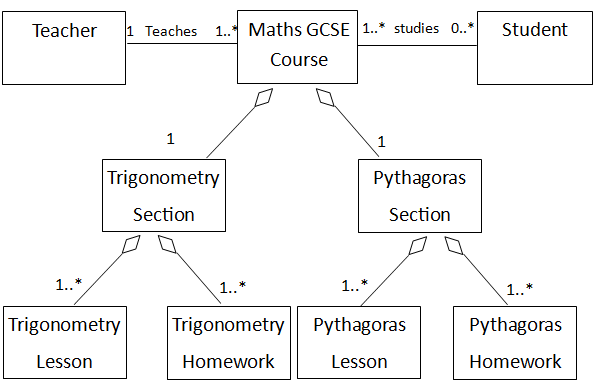
\includegraphics[width=\textwidth]{U:/git/COMP4Coursework2/Design/objectrelationships.png}
    \caption{The relationships between each of the objects in the proposed system} \label{fig:print_function_result}
\end{figure}

\subsection{Class Definitions}

\begin{center}
\begin{tabular}{|p{5cm}|} \hline
Course \\ \hline
Title \\
Subject \\ \hline
AddTitle \\ 
EditTitle \\
AddSubject \\
EditSubject \\ \hline
\end{tabular}
\end{center}

\begin{center}
\begin{tabular}{|p{5cm}|} \hline
Teacher \\ \hline
Surname \\
Title \\
Subject \\ \hline
AddSurname \\
EditSurname \\
AddTitle \\
EditTitle \\
AddSubject \\
EditSubject \\ \hline
\end{tabular}
\end{center}

\begin{center}
\begin{tabular}{|p{5cm}|} \hline
Student \\ \hline
FirstName \\
Surname \\
UserID \\
Password  \\ \hline
AddFirstName \\
EditFirstName \\
AddSurname \\
EditSurname \\
AddUserID \\
EditUserID \\
AddPassword \\
EditPassword \\ \hline
\end{tabular}
\end{center}

\begin{center}
\begin{tabular}{|p{5cm}|} \hline
Trigonometry Section \\ \hline
TrigonometryLesson \\
TrigonometryHomework \\ \hline
PresentTrigonometryLesson \\
SetTrigonometryHomework \\
MarkTrigonometryHomework \\ \hline
\end{tabular}
\end{center}

\begin{center}
\begin{tabular}{|p{5cm}|} \hline
Pythagoras Section \\ \hline
PythagorasLesson \\
PythagorasHomework \\ \hline
PresentPythagorasLesson \\
SetPythagorasHomework \\
MarkPythagorasHomework \\ \hline
\end{tabular}
\end{center}

\begin{center}
\begin{tabular}{|p{5cm}|} \hline
Trigonometry Lesson \\ \hline
Examples \\
Questions \\ \hline
DisplayExamples \\
GiveExampleAnswers \\
GiveQuestionAnswers \\ \hline
\end{tabular}
\end{center}

\begin{center}
\begin{tabular}{|p{5cm}|} \hline
Trigonometry Homework \\ \hline
Questions \\
Answers \\ \hline
SetQuestions \\
CheckAnswers \\
DisplayCorrectAnswers \\
OutputCorrectMessage \\
OutputDataTypeErrorMessage \\
SubmitScore \\ \hline
\end{tabular}
\end{center}

\begin{center}
\begin{tabular}{|p{5cm}|} \hline
Pythagoras Lesson \\ \hline
Examples \\
Questions \\ \hline
DisplayExamples \\
GiveExampleAnswers \\
GiveQuestionAnswers \\ \hline
\end{tabular}
\end{center}

\begin{center}
\begin{tabular}{|p{5cm}|} \hline
Pythagoras Homework \\ \hline
Questions \\
Answers \\ \hline
SetQuestions \\
CheckAnswers \\
DisplayCorrectAnswers \\
OutputCorrectMessage \\
OutputDataTypeErrorMessage \\
SubmitScore \\ \hline
\end{tabular}
\end{center}

\begin{center}
\begin{tabular}{|p{5cm}|} \hline
QuestionType \\ \hline
QuestionType \\
QuestionInput \\
QuestionOutput \\ \hline
InputSolution \\
CheckSolution \\
OutputError \\ \hline
\end{tabular}
\end{center}

\begin{center}
\begin{tabular}{|p{5cm}|} \hline
TextQuestion \\ \hline
QuestionInputText \\ 
QuestionOutput \\ \hline
InputSolutionText \\ 
CheckSolution \\
OutputError \\ \hline
\end{tabular}
\end{center}

\begin{center}
\begin{tabular}{|p{5cm}|} \hline
DragAndDropQuestion \\ \hline
QuestionDragImage \\ 
QuestionOutput \\ \hline
InputDragImage \\ 
CheckSolution \\
OutputError \\ \hline
\end{tabular}
\end{center}

\begin{center}
\begin{tabular}{|p{5cm}|} \hline
ImageQuestion \\ \hline
QuestionSelectButton \\ 
QuestionOutput \\ \hline
InputSolutionButton \\ 
CheckSolution \\
OutputError \\ \hline
\end{tabular}
\end{center}

\section{Prototyping}

\begin{figure}[H]
    \label{fig:print_function_result}\caption{Login Screen: The user inputs their username and password and selects log in.}
    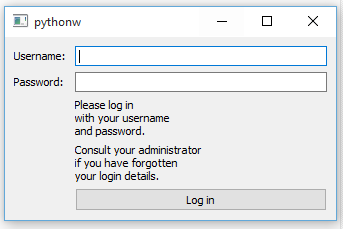
\includegraphics[width=\textwidth]{U:/git/COMP4Coursework2/Design/pyqt_figure_1}
\end{figure}

\begin{figure}[H]
    \label{fig:print_function_result}\caption{ErrorMessage2: If the user's input username or password is incorrect, this message will appear.}
    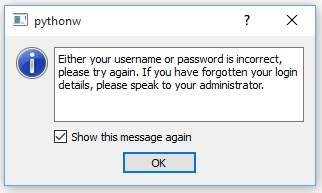
\includegraphics[width=\textwidth]{U:/git/COMP4Coursework2/Design/pyqt_figure_2}
\end{figure}

\begin{figure}[H]
    \label{fig:print_function_result}\caption{Student Home Screen: If the user's username is recognised as a student's name, the student version of the home screen will appear.}
    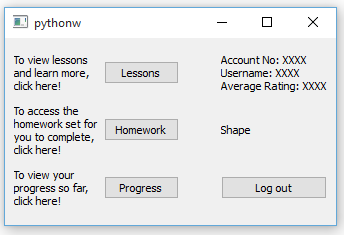
\includegraphics[width=\textwidth]{U:/git/COMP4Coursework2/Design/pyqt_figure_3}
\end{figure}

\begin{figure}[H]
    \label{fig:print_function_result}\caption{Lesson Topic Menu: Appears if the user selects the lessons button - displays the topics to choose from.}
    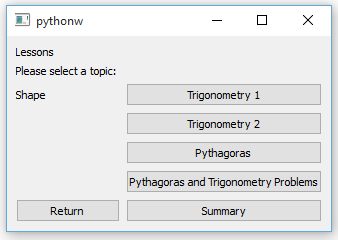
\includegraphics[width=\textwidth]{U:/git/COMP4Coursework2/Design/pyqt_figure_4}
\end{figure}

\begin{figure}[H]
    \label{fig:print_function_result}\caption{Lesson Menu: Will appear for any lesson topic selected, displaying the buttons for the topic specific lessons to choose from. Will look the same for each topic except for the button and window names.}
    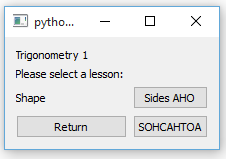
\includegraphics[width=\textwidth]{U:/git/COMP4Coursework2/Design/pyqt_figure_5}
\end{figure}

\begin{figure}[H]
    \label{fig:print_function_result}\caption{First Lesson Screen: Will appear with the lessons depending on which button was selected; all lessons will use a generic design plan.}
    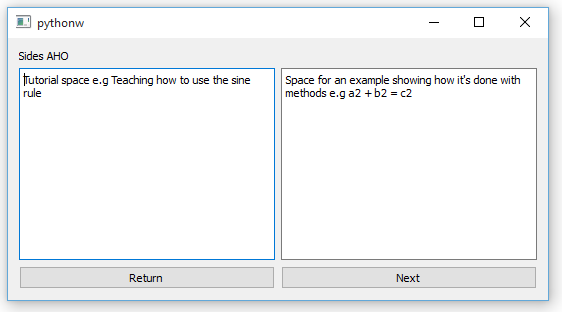
\includegraphics[width=\textwidth]{U:/git/COMP4Coursework2/Design/pyqt_figure_6}
\end{figure}

\begin{figure}[H]
    \label{fig:print_function_result}\caption{Second Lesson Screen: Appears once next has been selected from the previous screen, continuing a generic design plan and displaying the next examples.}
    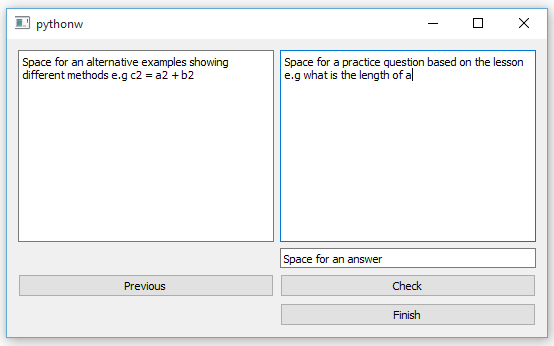
\includegraphics[width=\textwidth]{U:/git/COMP4Coursework2/Design/pyqt_figure_7}
\end{figure}

\begin{figure}[H]
    \label{fig:print_function_result}\caption{Homework Topic Menu: Appears if the user selects the homework button - displays the topics to choose from.}
    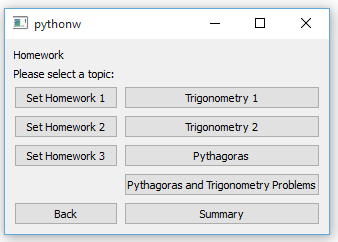
\includegraphics[width=\textwidth]{U:/git/COMP4Coursework2/Design/pyqt_figure_8}
\end{figure}

\begin{figure}[H]
    \label{fig:print_function_result}\caption{Homework Menu: Will appear for any homework topic selected, displaying the buttons for the topic specific homeworks to choose from. Will look the same for each topic except for the button and window names.}
    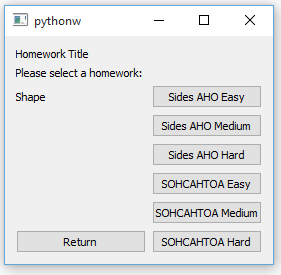
\includegraphics[width=\textwidth]{U:/git/COMP4Coursework2/Design/pyqt_figure_9}
\end{figure}

\begin{figure}[H]
    \label{fig:print_function_result}\caption{First Homework Screen: Will appear with the homework depending on which button was selected; all homeworks will use a generic design plan.}
    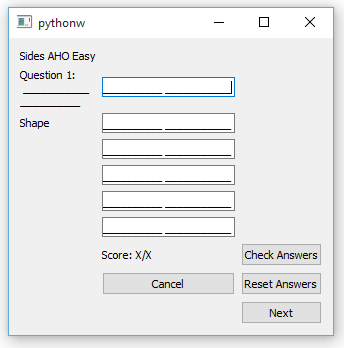
\includegraphics[width=\textwidth]{U:/git/COMP4Coursework2/Design/pyqt_figure_10}
\end{figure}

\begin{figure}[H]
    \label{fig:print_function_result}\caption{Second Homework Screen: Appears once next has been selected from the previous screen, continuing a generic design plan and displaying the next questions.}
    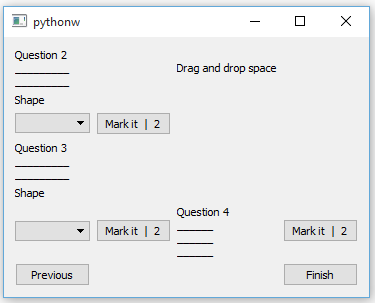
\includegraphics[width=\textwidth]{U:/git/COMP4Coursework2/Design/pyqt_figure_11}
\end{figure}

\begin{figure}[H]
    \label{fig:print_function_result}\caption{Individual User Progress Database: Appears if the user selects the progress button - displays their individual database in a table in the window.}
    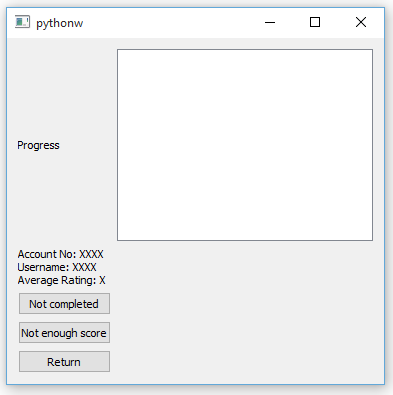
\includegraphics[width=\textwidth]{U:/git/COMP4Coursework2/Design/pyqt_figure_12}
\end{figure}

\begin{figure}[H]
    \label{fig:print_function_result}\caption{Administrator Account Home: If the user's username is recognised as an teacher's name, the administrator version of the home screen will appear.}
    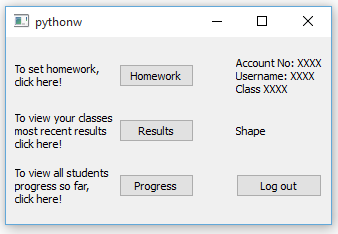
\includegraphics[width=\textwidth]{U:/git/COMP4Coursework2/Design/pyqt_figure_13}
\end{figure}

\begin{figure}[H]
    \label{fig:print_function_result}\caption{Homework Setting Topic Menu: Appears if the user selects the homework button - displays the topics to choose from to set as homework.}
    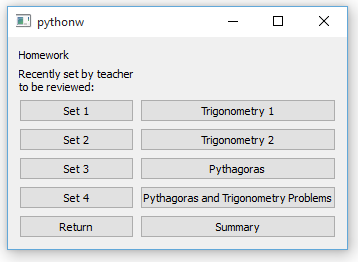
\includegraphics[width=\textwidth]{U:/git/COMP4Coursework2/Design/pyqt_figure_14}
\end{figure}

\begin{figure}[H]
    \label{fig:print_function_result}\caption{Homework Set Screen: Appears once a topic has been selected - once the set button is pressed this homework will be available on each student's homework to-do list.}
    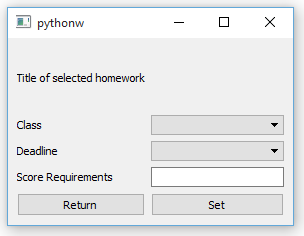
\includegraphics[width=\textwidth]{U:/git/COMP4Coursework2/Design/pyqt_figure_15}
\end{figure}

\begin{figure}[H]
    \label{fig:print_function_result}\caption{Results Menu: Appears if the user selects the results button - displays a list of buttons leading to homework recently completed that needs to be checked.}
    \includegraphics[width=\textwidth]{U:/git/COMP4Coursework2/Design/pyqt_figure_16}
\end{figure}

\begin{figure}[H]
    \label{fig:print_function_result}\caption{Class Results Database: Once a homework is selected from the previous screen, the database will appear showing all the results for that specific homework.}
    \includegraphics[width=\textwidth]{U:/git/COMP4Coursework2/Design/pyqt_figure_17}
\end{figure}

\begin{figure}[H]
    \label{fig:print_function_result}\caption{ErrorMessage3: Appears if the user inputs a wrong data type into an answer box on a homework - should be a decimal.}
    \includegraphics[width=\textwidth]{U:/git/COMP4Coursework2/Design/pyqt_figure_18}
\end{figure}

\begin{figure}[H]
    \label{fig:print_function_result}\caption{ErrorMessage3: Appears if the user inputs a wrong data type into an answer box on a homework - should be an intege.r}
    \includegraphics[width=\textwidth]{U:/git/COMP4Coursework2/Design/pyqt_figure_19}
\end{figure}

\begin{figure}[H]
    \label{fig:print_function_result}\caption{ErrorMessage3: Appears if the user inputs a wrong data type into an answer box on a homework - should be a string.}
    \includegraphics[width=\textwidth]{U:/git/COMP4Coursework2/Design/pyqt_figure_20}
\end{figure}

\begin{figure}[H]
    \label{fig:print_function_result}\caption{ErrorMessage4: Appears if the user gets the wrong answer on an answer box on a homework.}
    \includegraphics[width=\textwidth]{U:/git/COMP4Coursework2/Design/pyqt_figure_21}
\end{figure}

\section{Definition of Data Requirements}

\subsection{Identification of all data input items}

\begin{itemize}
	\item Log In Inputs:
	\begin{itemize}
		\item Username
		\item Password
	\end{itemize}
	\item Lesson Inputs:
	\begin{itemize}
		\item Lesson test answer
		\item Check answers button
	\end{itemize}
	\item Homework Set Inputs:
	\begin{itemize}
		\item Class
		\item Deadline
		\item Score Requirements
		\item Set homework button
	\end{itemize}
	\item Homework Inputs:
	\begin{itemize}
		\item Question 1a answer
		\item Question 1b answer
		\item Question 1c answer
		\item Question 1d answer
		\item Question 1e answer
		\item Question 1f answer
		\item Question 2 drop down selection
		\item Question 3 drop down selection
		\item Question 4 drag and drop inputs
		\item Submit answers button
		\item Homework Buttons:
		\begin{itemize}
			\item Reset answers button
			\item Mark answers button
		\end{itemize}
	\end{itemize}
	\item All Other Buttons:
	\begin{itemize}
		\item Log in button
		\item Student Version:
		\begin{itemize}
			\item Lesson button
			\item Homework button
			\item Progress button
			\item Lesson topic buttons	
			\item Lesson buttons
			\item Homework topic buttons
			\item Homework buttons
			\item Set homework buttons
		\end{itemize}
		\item Teacher Version:
		\begin{itemize}
			\item Homework button
			\item Results button
			\item Progress button
			\item Result selection buttons
			\item Feedback
		\end{itemize}
		\item Previous button
		\item Next button
		\item Return button
		\item Finish button
		\item OK button
		\item Log out button
	\end{itemize}
\end{itemize}

\subsection{Identification of all data output items}

\begin{itemize}
	\item Displays:
	\begin{itemize}
		\item All screens
		\item Hard-coded lesson examples
		\item Hard-coded homework questions
		\item Correct answers
	\end{itemize}
	\item Database:
	\begin{itemize}
		\item FirstName
		\item LastName
		\item TaskName
		\item OverallPercentageScore
		\item IndividualPercentageScore (For each question in a homework)
		\item Rating
		\item Feedback (From teacher to student)
	\end{itemize}
	\item Error Messages:
	\begin{itemize}
		\item ErrorMessage2
		\item ErrorMessage3 - Decimal
		\item ErrorMessage3 - Integer
		\item ErrorMessage3 - String
		\item ErrorMessage4
	\end{itemize}
	\item Displayed On Home:
	\begin{itemize}
		\item Account name
		\item Username
		\item Average rating (Student)
		\item Class (Teacher)
	\end{itemize}
\end{itemize}

\subsection{Explanation of how data output items are generated}

\begin{center}
\begin{tabular}{|p{4cm}|p{6cm}|} \hline
\textbf{Output} & \textbf{How it's generated} \\ \hline
Lesson Examples & These are hard-coded and will be saved as overrides in each lesson's subclass \\ \hline
Homework Examples & These are hard-coded and will be saved as overrides in each homework's subclass \\ \hline
Correct Answers & These will be generated using algorithms which will solve the same problem the user is trying to solve, find the answer, and display it \\ \hline
FirstName & This will be saved to the database once the administrator inputs the class names \\ \hline
LastName & This will be saved to the database once the administrator inputs the class names \\ \hline
TaskName & This will be hard-coded as an attribute in each subclass \\ \hline
OverallPercentageScore & When a homework task is submitted, algorithms will check how many answers were correct, and obtain a percentage from them, then calculate the average from them \\ \hline
IndividualPercentageScore & When a homework task is submitted, algorithms will check how many answers were correct, and obtain a percentage from each question from the average of each question's parts \\ \hline
Rating & This will be decided using selection statements depending on what the OverallPercentageScore is \\ \hline
Feedback & The administrator will manually input this and the user will then be able to see it on their individual results page \\ \hline
ErrorMessage2 & This is a hard-coded QErrorMessage() which will appear if the user inputs an incorrect username or password \\ \hline
ErrorMessage3 & These are hard-coded QErrorMessage()s which will appear if the user inputs an incorrect data type as an answer, depending on what the data type is supposed to be \\ \hline
\end{tabular}
\end{center}

\begin{center}
\begin{tabular}{|p{4cm}|p{6cm}|}  \hline
\textbf{Output} & \textbf{How it's generated} \\ \hline
ErrorMessage4 & This is a hard-coded QErrorMessage() which will appear if the user inputs an incorrect answer to a  homework question \\ \hline
Account Name & Will be a unique identifier saved by the system, only visible on the homescreens \\ \hline
Username & This is the same as the username used to log in, and will be obtained from the same place it's saved for validation, probably a notepad file \\ \hline
Average Rating & All of the user's past homework's ratings will be averaged and displayed on the homescreen \\ \hline
Class & This will be input by the administrator before inputting each students name \\ \hline
\end{tabular}
\end{center}

\subsection{Data Dictionary}

\begin{center}
\begin{tabular}{|p{3.4cm}|p{1.2cm}|p{2cm}|p{2cm}|p{2cm}|p{3.5cm}|}
\hline
\textbf{Name} & \textbf{Data Type} & \textbf{Length} & \textbf{Validation} & \textbf{Example Data} & \textbf{Comment} \\ \hline
UserID & Integer & 4 bits & 0001 to 9999 & 1546 & Unique to each user \\ \hline
Password & String and integers & 7 characters & letter followed by number followed by letter & f7h3j5f & The password generator uses mixed data types to avoid inappropriate passwords \\ \hline
FirstName & String & 15 characters & First letter upper case, rest lower case & John & Unique to each user, but could be shared by some \\ \hline
Surname & String & 25 characters & First letter upper case, rest lower case & Smith & Unique to each user, but could be shared by some \\ \hline
TaskName & String & 25 characters & & Trigonometry 2 & Hard-coded into the system \\ \hline
OverallPercentScore & Real & 3 characters & in range 0 - 100 & 76.5\% & The percentage of marks obtained in a test, decimal points allowed \\ \hline
\end{tabular}
\end{center}

\begin{center}
\begin{tabular}{|p{3.4cm}|p{1.2cm}|p{2cm}|p{2cm}|p{2cm}|p{3.5cm}|}
\hline
\textbf{Name} & \textbf{Data Type} & \textbf{Length} & \textbf{Validation} & \textbf{Example Data} & \textbf{Comment} \\ \hline
IndividualPercentScore & Real & 3 characters & in range 0 - 100 & 45.5\% & The percentage of marks for an individual question, field will only appear in separate table for individual tasks \\ \hline
Rating & Blob & 64 kilobytes & \ &  Green face graphic & Green, amber or red face graphic \\ \hline
Feedback & String & 500 characters & \ & Good work & This can consist of any characters as it is a personal message \\ \hline
AppointmentTime & Time & 5 characters & 24 hour format & 13:35 & Only relevant if the user has a true SeeAfterClass variable, set automatically bsed on the administrator's timetable but can be changed if necessary\\ \hline
SeeAfterClass & Boolean & 3 characters & Yes or No & Yes & If the user doesn't achieve a sufficient score, this variable will become true and alert the user \\ \hline
ErrorMessage1 & String & 50 characters & & Sorry, the name cannot have integers & An error message if the wrong data type is used to input a name \\ \hline
ErrorMessage2 & String & 50 characters & & Sorry, that is not a valid login & Tells the user if they have input the wrong username or password \\ \hline
ErrorMessage3 & String & 50 characters & & Please input a decimal, not an integer & Tells the user if their incorrect answer is the wrong data type \\ \hline
ErrorMessage4 & String & 50 characters & & That is incorrect, try one more time & Tells the user that their answer is incorrect and gives them one more attempt \\ \hline
CorrectAnswer & Integer, Real, String & 5 characters & Must be a decimal or whole number, or text & 25.5cm & Gives the user the correct answer if they get the question wrong too many times \\ \hline
\end{tabular}
\end{center}

\begin{center}
\begin{tabular}{|p{3.4cm}|p{1.2cm}|p{2cm}|p{2cm}|p{2cm}|p{3.5cm}|}
\hline
\textbf{Name} & \textbf{Data Type} & \textbf{Length} & \textbf{Validation} & \textbf{Example Data} & \textbf{Comment} \\ \hline
Login data & String & 25 characters & & johnsmith1, f8j4h6k & The login information saved in the system to be loaded and checked with the user's inputs \\ \hline
Task data & String & 100 characters & & Trigonometry - sin rule, Level 7, Trigonometry & Contains all the information about the task, what difficulty it is, what type it is etc. \\ \hline
Set answers & Integer, Real, String & 5 characters & Must be a decimal or whole number, or text if in a text box & 45{$^o$} & Contains all the set answers for some of the tasks \\ \hline
Calculated answers & Integer, Real & 5 characters & Must be the same solution as the algorithm & 29.8 & Contains algorithms which find and validate the solution for randomly generated tasks \\ \hline
Account name & Integer & 4 characters & Must be a string of 4 integers, 0 - 9 & 1357 & This is the unique identifier for the database \\ \hline
Average rating & Blob & 1 blob & Will be a green, amber or red face & Green face blob & This is the rating from the average rating of each student's completed homework so far \\ \hline
Class & String & 3 - 6 characters & Must be the name of the class, same as is in the centre's system & 10A & Is input with the student names \\ \hline
\end{tabular}
\end{center}

\subsection{Identification of appropriate storage media}

My system files will need to be stored on the school's local server, as every part will need to be accessible from every computer, to save the teacher having to log into every computer one at a time to check work. this way, every computer can access every account, and if they have the permissions, every part of the database. If necessary, some files can be backed up onto an individual computer in the system, or onto a USB stick. As a result, all users and administrators will be able to share the files and use them at the same time.

\section{Database Design}

\subsection{Normalisation}

\subsubsection{ER Diagrams}

\begin{figure}[H]
    \label{fig:print_function_result}
    \includegraphics[width=\textwidth]{U:/git/COMP4Coursework2/Design/er_diagram}
\end{figure}

\subsubsection{Entity Descriptions}

\begin{center}
\begin{tabular}{|p{3cm}|p{4cm}|p{4cm}|p{3cm}|} \hline
\textbf{Entity} & \textbf{Description} & \textbf{Attributes} & \textbf{Key} \\ \hline
Student & Each record shows how many results a student receives, and which class they are in & \textbf{Student}(\underline{StudentID}, \underline{ClassID}) & Primary Key(StudentID, ClassID) \\ \hline
Class & Shows which students are in the class and the teacher of that class, and how much homework the class has been set & \textbf{Class}(\underline{ClassID}, TeacherID) & Primary Key(ClassID) \\ \hline
Homework & Shows who each homework has been set for, and the results if the homework has been completed & \textbf{Homework}(\underline{HomeworkID}, HomeworkSet, HomeworkResults) & Primary Key(HomeworkID) \\ \hline 
HomeworkSet & Shows who has been set the homework, when, and how many times/how long for & \textbf{HomeworkSet}(\underline{ClassID}, \underline{HomeworkID}, DueDate, SetDate) & Primary Key(ClassID, HomeworkID) \\ \hline
HomeworkResults & This record contains all of the results for a completed homework & \textbf{HomeworkResults} (\underline{HomeworkID}, \underline{StudentID}, \underline{QuestionID}, Rating, CompletedDate) & Primary Key(HomeworkID, StudentID, QuestionID) \\ \hline
Question & Shows how many questions were in a homework, and the percentage which are correct in each students results & \textbf{Question}(\underline{HomeworkID}, \underline{QuestionID}, QuestionText, Choice1, Choice2, ChoiceX, CorrectAnswer, TypeOfQuestion) & Primary Key(HomeworkID, QuestionID) \\ \hline
\end{tabular}
\end{center}

\subsubsection{UNF to 3NF}

\textbf{Unnormalised: }

\begin{center}
\begin{tabular}{|p{4cm}|} \hline
AccountID \\
UserID \\
ClassID
FirstName \\
LastName \\
TaskName \\
OverallPercentScore \\
IndividualPercentScore \\
Rating \\
Feedback \\ \hline
\end{tabular}
\end{center}

\textbf{1st Normalised Form: }

\begin{center}
\begin{tabular}{|p{4cm}|p{3cm}|} \hline
\textbf{Repeating Attributes} & \textbf{Non-repeating Attributes} \\ \hline
\textbf{\underline{UserID}} & \textbf{\underline{AccountID}} \\
\textbf{\underline{ClassID}} & \\
\textbf{\underline{TaskName}} & \\
FirstName & \\
LastName & \\
OverallPercentScore & \\
IndividualPercentScore & \\
Feedback & \\
Rating & \\ \hline
\end{tabular}
\end{center}

\textbf{2nd Normalised Form: }

\begin{center}
\begin{tabular}{|p{4cm}|p{3cm}|} \hline
\textbf{Repeating Attributes} & \textbf{Non-repeating Attributes} \\ \hline
\textbf{\underline{ClassID}} & \textbf{\underline{AccountID}} \\
\textbf{\underline{UserID}} & \\
FirstName & \\
LastName & \\
 & \\
\textbf{\underline{TaskName}} & \\
OverallPercentScore & \\
IndividualPercentScore & \\
Feedback & \\
Rating & \\ \hline
\end{tabular}
\end{center}

\textbf{3rd Normalised Form: }

\begin{center}
\begin{tabular}{|p{4cm}|p{3cm}|} \hline
\textbf{Repeating Attributes} & \textbf{Non-repeating Attributes} \\ \hline
\textbf{\underline{ClassID}} & \textbf{\underline{AccountID}} \\
\textbf{\underline{UserID}} & \\
FirstName & \\
LastName & \\
 & \\
\textbf{\underline{TaskName}} & \\
\underline{IndividualPercentScore} & \\
& \\
\textbf{\underline{IndividualPercentScore}} & \\
\underline{OverallPercentScore} & \\
& \\
\textbf{\underline{OverallPercentScore}} & \\
Rating & \\
Feedback & \\ \hline
\end{tabular}
\end{center}

\subsection{SQL Queries}

\begin{center}
\begin{tabular}{|p{8cm}|p{6cm}|} \hline
\textbf{SQL Query (Python Format)} & \textbf{Description} \\ \hline
sql = """create table Student & This is the SQL statement which \\ 
(UserID integer, & creates the initial table called \\
FirstName text, & Student, with all of the attributes \\
LastName text, & that need to be displayed to the users \\
TaskName text, & in the database \\
OverallPercentScore real, & \\
IndividualPercentScore real, &\\
Rating blob, & \\
Feedback text, & \\
primary key(UserID))""" & \\ \hline
"""insert into Student & This query adds values to the \\
(FirstName, LastName, UserID) values ('\{0\}', '\{1\}', '\{2\}') & FirstName, LastName and UserID \\
""".format(FirstName, LastName, UserID) & fields when the administrator adds names to the system \\ \hline
"""select * from Student & This query is for student use and it \\
where TaskName = '\{0\}' and UserID = '\{1\}' & fetches all of the database information \\
""".format(TaskName, UserID) & for that user for a specific homework they have completed \\ \hline
"""select * from Class & This query is for teacher use and it \\
where TaskName = '\{0\}' and ClassID = '\{1\}' & fetches all of the records saved for an\\
""".format(TaskName, ClassID) & entire class for a specific homework \\ \hline
"""select * from Class & This query will fetch all of the records \\
where StudentID = '\{0\}'""".format(StudentID) & stored for a specific student, for teacher use \\ \hline
"""select * from Class & This query can be used by the teacher \\
where TaskName = '\{0\}' and Rating = '\{1\}' & to search for all homework done in a \\
""".format(TaskName, Rating) & class which has not been done to a sufficient standard \\ \hline
"""select * from Student & This query will select all of the \\
where StudentID = '\{0\}' and Rating = '\{1\}' & homework done by one student which \\
""".format(StudentID, Rating) & has not been done to a sufficient standard \\ \hline
"""update Student & This query will update the database \\
OverallPercentScore = '\{0\}' & with the results when a student \\
IndividualPercentScore = '\{1\}' & completes a homework \\
Rating = '\{2\}' & \\
where StudentID = '\{3\}' and TaskName = '\{4\}' & \\
""".format(OverallPercentScore, IndividualPercentScore, Rating, StudentID, TaskName) & \\ \hline
\end{tabular}
\end{center}

\begin{center}
\begin{tabular}{|p{8cm}|p{6cm}|} \hline
\textbf{SQL Query (Python Format)} & \textbf{Description} \\ \hline
"""update Student & This query will update the records \\
Feedback = '\{0\}' & for a student when the \\
where StudentID = '\{1\}' and TaskName = '\{2\}' & teacher manually gives them \\
""".format(Feedback, StudentID, TaskName) & feedback \\ \hline
\end{tabular}
\end{center}

\section{Security and Integrity of the System and Data}

\subsection{Security and Integrity of Data}

As this system will store a small amount of personal data (FirstName, LastName, ClassID), the Data Protection Act of 1998 must be followed. Therefore the data must be kept up to date, and a way of editing the FirstName, LastName and ClassID records will be included to ensure that wrong data is not forced to be kept permanently, should it be input by mistake. To ensure that the data is not kept for longer than the DPA says it should be, any old data will be searched for and deleted whenever the system is started, should it be found. Furthermore, checks shall be implemented to ensure key data fields are not left empty, in order to maintain referential integrity. The only possible way to view the data stored by my system will be on the visual database in the graphical user interface, which will only be accessible following the input of a correct username and password. Finally, all of the data stored will be valid and feasible as drop down menus, and data type relevant error messages will be used to ensure the user is given a fair chance to input answers.

\subsection{System Security}

In order to prevent theft of information and tampering, all information in the system will only be accessible by providing a username and password, and each user will only be allowed to view data relevant to their own progression. Students will not be able to change any information in the database, but teachers will, if they accidentally include a typo when inputting names into the system. Furthermore, the number of people with access to the system will be limited, and those with key access trusted as professional teachers. The database will be encrypted to avoid people somehow accessing the database information by some other means, although only names will be stored as personal information. Lastly, all of the names input into the system will have a validation check to ensure they do not accidentally include numbers, extra capital letters, not enough capital letters or other characters not in the alphabet. Because the names stored will fall under the Data Protection Act, I will ensure that no data is sent to other countries, or even anywhere at all outside of the school, that the data is secure and only accessible by authorised people, that it is only stored by the school, that the data can be updated and destroyed to ensure protection, and that only necessary data will be collected in the first place.

\section{Validation}

\begin{center}
\begin{tabular}{|p{2cm}|p{3cm}|p{4cm}|p{4cm}|} \hline
\textbf{Item} & \textbf{Example} & \textbf{Validation applied} & \textbf{Comments} \\ \hline
ClassID & 10A & Presence check & The ClassID is the same as the classes actual class name, so no validation is required \\ \hline
FirstName & John & Data type check: First letter, capital, rest lower case, all string, no spaces & Checks that the name given is in fact a name \\ \hline
LastName & Smith & Data type check: First letter, capital, rest lower case, all string, no spaces & Checks that the name given is in fact a name \\ \hline
Username & User \ 1 & Format check: First 4 letters of LastName followed by a number. Validation check - Check it's in the system as a valid username & This ensures that the username is in the right format before checking if it's recognised as a valid username \\ \hline
Password & f5h3d7h & Format check: letter, number, letter, number, letter, number, letter, all lower case. Validation check - Check it's in the system and matches the username input beforehand & The password is randomly generated and attached to the username, in that format to avoid any inappropriate words being generated \\ \hline
Text answer input & 7 & ValueErrorCheck - integer & Checks that the value input is the correct data type \\ \hline
Text answer input & 7.5 & ValueErrorCheck - decimal & Checks that the value input is the correct data type \\ \hline
Text answer input & seven & ValueErrorCheck - string & Checks that the value input is the correct data type  \\ \hline
ComboBox answer input & select 5 & Presence check & Checks that an option has actually been selected \\ \hline
Drag and drop answer input & all pictures dropped onto shape & Presence check & Checks to see if all of the drag icons have been dropped into the corresponding spaces \\ \hline
Correct & True & Presence check & This boolean corresponds to every answer and says whether or not it is correct \\ \hline
\end{tabular}
\end{center}

\begin{center}
\begin{tabular}{|p{2cm}|p{3cm}|p{4cm}|p{4cm}|} \hline
\textbf{Item} & \textbf{Example} & \textbf{Validation applied} & \textbf{Comments} \\ \hline
Class selected & 10A and & Presence check & Makes sure a class has been selected from the combo box to set the homework for \\ \hline
Deadline & 14/12/15 & Presence check & Makes sure a date within a given set of boundaries has been selected from the combo box \\ \hline
Score Requirements & 75\% & Presence check & Makes sure a score percentage has been selected from the combo box \\ \hline
\end{tabular}
\end{center}

\section{Testing}

\begin{landscape}
\subsection{Outline Plan}

\begin{center}
    \begin{tabular}{|p{2cm}|p{5cm}|p{5cm}|p{4cm}|}
        \hline
        \textbf{Test Series} & \textbf{Purpose of Test Series} & \textbf{Testing Strategy} & \textbf{Strategy Rationale}\\ \hline
        1 & Test the connections between all of the buttons on the user interfaces & Top-down testing & Each button will be tested to make sure it connects to the right screen \\ \hline
        2 & Test all of the input spaces & Bottom-up testing & Each input will be tested once it is developed \\ \hline
        3 & Test all information is stored in the correct space in the database & Black box testing & The database will be viewed in a database viewer to ensure that SQL queries are working and data is being stored in the database once they have been developed \\ \hline
	4 & Test all of the mathematical algorithms to make sure that the program gives the correct output and marks & White box testing & Each algorithm will be tested once it is developed \\ \hline
	5 & Test that the system fulfils the clients request & Acceptance testing & The system will be developed once it is completed to a usable standard \\ \hline
    \end{tabular}
\end{center}

\subsection{Detailed Plan}

\begin{center}
    \begin{longtable}{|p{1.5cm}|p{2.5cm}|p{2.5cm}|p{2cm}|p{2cm}|p{2cm}|p{2cm}|p{2cm}|}
        \hline
        \textbf{Test Series} & \textbf{Purpose of Test} & \textbf{Test Description} & \textbf{Test Data} & \textbf{Test Data Type (Normal/ Erroneous/ Boundary)} & \textbf{Expected Result} & \textbf{Actual Result} & \textbf{Evidence}\\ \hline
1.001 & To test the student log in button on the first menu functions as intended & This should link to the student menu screen & Click the log in button & Normal & The student account screen should be displayed & & \\ \hline
1.002 & To test the teacher log in button on the first menu functions as intended & This should link to the administrator menu screen & Click the log in button & Normal & The administrator account screen should be displayed & & \\ \hline
1.003 & To test the lessons button on the student account screen functions as intended & This should link to the lesson topic menu screen & Click the lessons button & Normal & The lesson topic menu should be displayed & & \\ \hline
1.004 & To test the homework button on the student account screen functions as intended & This should link to the homework topic menu screen & Click the homework button & Normal & The homework topic menu should be displayed & & \\ \hline
1.005 & To test the progress button on the student account screen functions as intended & This should link to the student's personal database display screen & Click the progress button & Normal & The student's personal database screen should be displayed & & \\ \hline
1.006 & To test the log out button on the student account screen functions as intended & This should close down the entire program & Click the log out button & Normal & The program should stop & & \\ \hline
1.007 & To test the Trigonometry 1 button on the lesson topic menu screen functions as intended & This should link to the trigonometry 1 menu screen & Click the Trigonometry 1 button & Normal & The topic's menu screen should be displayed & & \\ \hline
1.008 & To test the Trigonometry 2 button on the lesson topic menu screen functions as intended & This should link to the trigonometry 2 menu screen & Click the Trigonometry 2 button & Normal & The topic's menu screen should be displayed & & \\ \hline
1.009 & To test the Pythagoras button on the lesson topic menu screen functions as intended & This should link to the pythagoras menu screen & Click the Pythagoras button & Normal & The topic's menu screen should be displayed & & \\ \hline
1.010 & To test the Pythagoras and Trigonometry Problems button on the lesson topic menu screen functions as intended & This should link to the trigonometry and pythagoras problems menu screen & Click the Pythaogras and Trigonometry Problems button & Normal & The topic's menu screen should be displayed & & \\ \hline
1.011 & To test the Summary button on the lesson topic menu screen functions as intended & This should link to the summary menu screen & Click the Summary button & Normal & The topic's menu screen should be displayed & & \\ \hline
1.012 & To test the return button on the lesson topic menu functions as intended & This should link back to the student account screen & Click the return button & Normal & The student account screen should be displayed & & \\ \hline
1.013 & To test the Sides button on the Trigonometry 1 lesson menu functions as intended & This should link to the screen for the first page of the sides lesson & Click the Sides button & Normal & The first sides lesson screen should be displayed & & \\ \hline
1.014 & To test the SOHCAHTOA button on the Trigonometry 1 lesson menu functions as intended & This should link to the screen for the first page of the SOHCAHTOA lesson & Click the SOHCAHTOA button & Normal & The first SOHCAHTOA lesson screen should be displayed & & \\ \hline
1.015 & To test the return button on the Trigonometry 1 menu functions as intended & This should link back to the lesson topic menu screen & Click the return button & Normal & The lesson topic menu should be displayed & & \\ \hline
1.016 & To test the Finding Angles button on the Trigonometry 2 lesson menu functions as intended & This should link to the screen for the first page of the finding angles lesson & Click the Finding angles button & Normal & The first finding angles lesson screen should be displayed & & \\ \hline
1.017 & To test the Inverted Angles button on the Trigonometry 2 lesson menu functions as intended & This should link to the screen for the first page of the inverted angles lesson & Click the Inverted angles button & Normal & The first inverted angles lesson screen should be displayed & & \\ \hline
1.018 & To test the 3D Trigonometry button on the Trigonometry 2 lesson menu functions as intended & This should link to the screen for the first page of the 3D Trigonometry lesson & Click the 3D Trigonometry button & Normal & The first 3D trigonometry lesson screen should be displayed & & \\ \hline
1.019 & To test the return button on the Trigonometry 2 menu functions as intended & This should link back to the lesson topic menu screen & Click the return button & Normal & The lesson topic menu should be displayed & & \\ \hline
1.020 & To test the Pythagoras Theorem button on the Pythagoras lesson menu functions as intended & This should link to the screen for the first page of the pythagoras theorem lesson & Click the pythagoras theorem button & Normal & The first pythagoras theorem lesson screen should be displayed & & \\ \hline
1.021 & To test the 3D Pythagoras button on the Pythagoras lesson menu functions as intended & This should link to the screen for the first page of the 3D pythagoras lesson & Click the 3D pythagoras button & Normal & The first 3D pythagoras lesson screen should be displayed & & \\ \hline
1.022 & To test the return button on the Pythagoras menu functions as intended & This should link back to the lesson topic menu screen & Click the return button & Normal & The lesson topic menu should be displayed & & \\ \hline
1.023 & To test the Easy Pythagoras and Trigonometry Problems button on the Trigonometry and Pythagoras Problems lesson menu functions as intended & This should link to the screen for the first page of the easy pythagoras and trigonometry problems lesson & Click the easy pythagoras and trigonometry problems button & Normal & The first easy pythagoras and trigonometry problems lesson screen should be displayed & & \\ \hline
1.024 & To test the Medium Pythagoras and Trigonometry Problems button on the Trigonometry and Pythagoras Problems lesson menu functions as intended & This should link to the screen for the first page of the medium pythagoras and trigonometry problems lesson & Click the medium pythagoras and trigonometry problems button & Normal & The first medium pythagoras and trigonometry problems lesson screen should be displayed & & \\ \hline
1.025 & To test the Hard Pythagoras and Trigonometry Problems button on the Trigonometry and Pythagoras Problems lesson menu functions as intended & This should link to the screen for the first page of the hard pythagoras and trigonometry problems lesson & Click the hard pythagoras and trigonometry problems button & Normal & The first hard pythagoras and trigonometry problems lesson screen should be displayed & & \\ \hline
1.026 & To test the return button on the Pythagoras and Trigonometry Problems menu functions as intended & This should link back to the lesson topic menu screen & Click the return button & Normal & The lesson topic menu should be displayed & & \\ \hline
1.027 & To test the Revise Trigonometry 1 button on the Summary lesson menu functions as intended & This should link to the screen for the first page of the revise trigonometry 1 lesson & Click the revise trigonometry 1 button & Normal & The first revise trigonometry 1 lesson screen should be displayed & & \\ \hline
1.028 & To test the Revise Trigonometry 2 button on the Summary lesson menu functions as intended & This should link to the screen for the first page of the revise trigonometry 2 lesson & Click the revise trigonometry 2 button & Normal & The first revise trigonometry 2 lesson screen should be displayed & & \\ \hline
1.029 & To test the Revise Trigonometry 3 button on the Summary lesson menu functions as intended & This should link to the screen for the first page of the revise trigonometry 3 lesson & Click the revise trigonometry 3 button & Normal & The first revise trigonometry 3 lesson screen should be displayed & & \\ \hline
1.030 & To test the return button on the Summary menu functions as intended & This should link back to the lesson topic menu screen & Click the return button & Normal & The lesson topic menu should be displayed & & \\ \hline
%1.031 & sides aho return button
%1.032 & sides aho next button
%1.033 & sides aho previous button
%1.034 & sides aho check button
%1.035 & sides aho finish button
%1.036 & SOHCAHTOA return button
%1.037 & SOHCAHTOA next button
%1.038 & SOHCAHTOA previous button
%1.039 & SOHCAHTOA check button
%1.040 & SOHCAHTOA finish button
%1.041 & Finding angles return button
%1.042 & Finding angles next button
%1.043 & Finding angles previous button
%1.044 & Finding angles check button
%1.045 & Finding angles finish button
%1.046 & inverted angles return button
%1.047 & inverted angles next button
%1.048 & inverted angles previous button
%1.049 & inverted angles check button
%1.050 & inverted angles finish button
%1.051 & 3D trig return button
%1.052 & 3D trig next button
%1.053 & 3D trig previous button
%1.054 & 3D trig check button
%1.055 & 3D trig finish button
%1.056 & pythag theorem return button
%1.057 & pythag theorem next button
%1.058 & pythag theorem previous button
%1.059 & pythag theorem check button
%1.060 & pythag theorem finish button
%1.061 & 3D pythag return button
%1.062 & 3D pythag next button
%1.063 & 3D pythag previous button
%1.064 & 3D pythag check button
%1.065 & 3D pythag finish button
%1.066 & pytrig easy return button
%1.067 & pytrig easy next button
%1.068 & pytrig easy previous button
%1.069 & pytrig easy check button
%1.070 & pytrig easy finish button
%1.071 & pytrig medium return button
%1.072 & pytrig medium next button
%1.073 & pytrig medium previous button
%1.074 & pytrig medium check button
%1.075 & pytrig medium finish button
%1.076 & pytrig hard return button
%1.077 & pytrig hard next button
%1.078 & pytrig hard previous button
%1.079 & pytrig hard check button
%1.080 & pytrig hard finish button
%1.081 & revise trig 1 return button
%1.082 & revise trig 1 next button
%1.083 & revise trig 1 previous button
%1.084 & revise trig 1 check button
%1.085 & revise trig 1 finish button
%1.086 & revise trig 2 return button
%1.087 & revise trig 2 next button
%1.088 & revise trig 2 previous button
%1.089 & revise trig 2 check button
%1.090 & revise trig 2 finish button
%1.091 & revise trig 3 return button
%1.092 & revise trig 3 next button
%1.093 & revise trig 3 previous button
%1.094 & revise trig 3 check button
%1.095 & revise trig 3 finish button
%1.096 & Set homework selection button
%1.097 & Trig 1 button
%1.098 & Trig 2 button
%1.099 & Pythag button
%1.100 & Pythag and trig button
%1.101 & Summary button
%1.102 & homework menu return button
%1.103 & Sides aho easy button
%1.104 & Sides aho medium button
%1.105 & sides aho hard button
%1.106 & SOHCAHTOA easy button
%1.107 & SOHCAHTOA medium button
%1.108 & SOHCAHTOA hard butotn
%1.109 & Trig 1 menu return button
%1.110 & Finding angles easy button
%1.111 & fa medium button
%1.112 & fa hard button
%1.113 & inverted angles easy button
%1.114 & ia medium button
%1.115 & ia hard button
%1.116 & 3D trig easy button
%1.117 & 3D trig medium button
%1.118 & 3D trig hard button
%1.119 & trig 2 menu return button
%1.120 & Pythag theorem easy button
%1.121 & pt medium button
%1.122 & pt hard button
%1.123 & 3D pythag easy button
%1.124 & 3D pythag medium button
%1.125 & 3D pythag hard button
%1.126 & pythagoras menu return button
%1.127 & Trig and pythag problems easy button
%1.128 & t + p p medium button
%1.129 & t + p p hard button
%1.130 & t + p p return button
%1.131 & easy summary button
%1.132 & medium summary button
%1.133 & hard summary button
%1.134 & summary return button
%1.135 & SIDES AHO EASY cancel button
%1.136 & sides aho check answers button
%1.137 & sides aho reset answers button
%1.138 & sides aho next button
%1.139 & sides aho mark it button 1
%1.140 & sides aho mark it button 2
%1.141 & sides aho mark it button 3
%1.142 & sides aho previous button
%1.143 & sides aho finish button
%1.144 & SIDES AHO MEDIUM cancel button
%1.145 & sides aho check answers button
%1.146 & sides aho reset answers button
%1.147 & sides aho next button
%1.148 & sides aho mark it button 1
%1.149 & sides aho mark it button 2
%1.150 & sides aho mark it button 3
%1.151 & sides aho previous button
%1.152 & sides aho finish button
%1.153 & SIDES AHO HARD cancel button
%1.154 & sides aho check answers button
%1.155 & sides aho reset answers button
%1.156 & sides aho next button
%1.157 & sides aho mark it button 1
%1.158 & sides aho mark it button 2
%1.159 & sides aho mark it button 3
%1.160 & sides aho previous button
%1.161 & sides aho finish button
%1.162 & SOHCAHTOA EASY cancel button
%1.163 &  check answers button
%1.164 & reset answers button
%1.165 &  next button
%1.166 &  mark it button 1
%1.167 &  mark it button 2
%1.168 &  mark it button 3
%1.169 &  previous button
%1.170 & finish button
%1.171 & SOHCAHTOA MEDIUM cancel button
%1.172 & sides aho check answers button
%1.173 & sides aho reset answers button
%1.174 & sides aho next button
%1.175 & sides aho mark it button 1
%1.176 & sides aho mark it button 2
%1.177 & sides aho mark it button 3
%1.178 & sides aho previous button
%1.179 & sides aho finish button
%1.180 & SOHCAHTOA HARD cancel button
%1.181 & sides aho check answers button
%1.182 & sides aho reset answers button
%1.183 & sides aho next button
%1.184 & sides aho mark it button 1
%1.185 & sides aho mark it button 2
%1.186 & sides aho mark it button 3
%1.187 & sides aho previous button
%1.188 & sides aho finish button
%1.189 & FINDING ANGLES EASY cancel button
%1.190 & sides aho check answers button
%1.191 & sides aho reset answers button
%1.192 & sides aho next button
%1.193 & sides aho mark it button 1
%1.194 & sides aho mark it button 2
%1.195 & sides aho mark it button 3
%1.196 & sides aho previous button
%1.197 & sides aho finish button
%1.198 & FINDING ANGLES MEDIUM cancel button
%1.199 & sides aho check answers button
%1.200 & sides aho reset answers button
%1.201 & sides aho next button
%1.202 & sides aho mark it button 1
%1.203 & ides aho mark it button 2
%1.204 & sides aho mark it button 3
%1.205 & sides aho previous button
%1.206 & sides aho finish button
%1.207 & FINDING ANGLES HARD cancel button
%1.208 & sides aho check answers button
%1.209 & sides aho reset answers button
%1.210 & sides aho next button
%1.211 & sides aho mark it button 1
%1.212 & sides aho mark it button 2
%1.213 & sides aho mark it button 3
%1.214 & sides aho previous button
%1.215 & sides aho finish button
%1.216 & INVERTED ANGLES EASY cancel button
%1.217 & sides aho check answers button
%1.218 & sides aho reset answers button
%1.219 & sides aho next button
%1.220 & sides aho mark it button 1
%1.221 & sides aho mark it button 2
%1.222 & sides aho mark it button 3
%1.223 & sides aho previous button
%1.224 & sides aho finish button
%1.225 & INVERTED ANGLES MEDIUM cancel button
%1.226 & sides aho check answers button
%1.227 & sides aho reset answers button
%1.228 & sides aho next button
%1.229 & sides aho mark it button 1
%1.230 & sides aho mark it button 2
%1.231 & sides aho mark it button 3
%1.232 & sides aho previous button
%1.233 & sides aho finish button
%1.234 & INVERTED ANGLES HARD cancel button
%1.235 & sides aho check answers button
%1.236 & sides aho reset answers button
%1.237 & sides aho next button
%1.238 & sides aho mark it button 1
%1.239 & sides aho mark it button 2
%1.240 & sides aho mark it button 3
%1.241 & sides aho previous button
%1.242 & sides aho finish button
%1.243 & 3D TRIG EASY cancel button
%1.244 &  check answers button
%1.245 & sides aho reset answers button
%1.246 & sides aho next button
%1.247 & sides aho mark it button 1
%1.248 & sides aho mark it button 2
%1.249 & sides aho mark it button 3
%1.250 & sides aho previous button
%1.251 & sides aho finish button
%1.252 & 3D TRIG MEDIUM cancel button
%1.253 & sides aho check answers button
%1.254 & sides aho reset answers button
%1.255 & sides aho next button
%1.256 & sides aho mark it button 1
%1.257 & sides aho mark it button 2
%1.258 & sides aho mark it button 3
%1.259 & sides aho previous button
%1.260 & sides aho finish button
%1.261 & 3D TRIG HARD cancel button
%1.262 & sides aho check answers button
%1.263 & sides aho reset answers button
%1.264 & sides aho next button
%1.265 & sides aho mark it button 1
%1.266 & sides aho mark it button 2
%1.267 & sides aho mark it button 3
%1.268 & sides aho previous button
%1.269 & sides aho finish button
%1.270 & PYTHAG THEOREM EASY cancel button
%1.271 & sides aho check answers button
%1.272 & sides aho reset answers button
%1.273 & sides aho next button
%1.274 & sides aho mark it button 1
%1.275 & sides aho mark it button 2
%1.276 & sides aho mark it button 3
%1.277 & sides aho previous button
%1.278 & sides aho finish button
%1.279 & PYTHAG THEOREM MEDIUM cancel button
%1.280 & sides aho check answers button
%1.281 & sides aho reset answers button
%1.282 & sides aho next button
%1.283 & sides aho mark it button 1
%1.284 & sides aho mark it button 2
%1.285 & sides aho mark it button 3
%1.286 & sides aho previous button
%1.287 & sides aho finish button
%1.288 & PYTHAG THEOREM HARD cancel button
%1.289 & sides aho check answers button
%1.290 & sides aho reset answers button
%1.291 & sides aho next button
%1.292 & sides aho mark it button 1
%1.293 & sides aho mark it button 2
%1.294 & sides aho mark it button 3
%1.295 & sides aho previous button
%1.296 & sides aho finish button
%1.297 & 3D PYTHAG EASY cancel button
%1.298 & sides aho check answers button
%1.299 & sides aho reset answers button
%1.300 & sides aho next button
%1.301 & sides aho mark it button 1
%1.302 & sides aho mark it button 2
%1.303 & sides aho mark it button 3
%1.304 & sides aho previous button
%1.305 & sides aho finish button
%1.306 & 3D PYTHAG MEDIUM cancel button
%1.307 & sides aho check answers button
%1.308 & sides aho reset answers button
%1.309 & sides aho next button
%1.310 & sides aho mark it button 1
%1.311 & sides aho mark it button 2
%1.312 & sides aho mark it button 3
%1.313 & sides aho previous button
%1.314 & sides aho finish button
%1.315 & 3D PYTHAG HARD cancel button
%1.316 & sides aho check answers button
%1.317 & sides aho reset answers button
%1.318 & sides aho next button
%1.319 & sides aho mark it button 1
%1.320 & sides aho mark it button 2
%1.321 & sides aho mark it button 3
%1.322 & sides aho previous button
%1.323 & sides aho finish button
%1.324 & sides aho cancel button
%1.325 & sides aho check answers button
%1.326 & sides aho reset answers button
%1.327 & sides aho next button
%1.328 & sides aho mark it button 1
%1.329 & sides aho mark it button 2
%1.330 & sides aho mark it button 3
%1.331 & sides aho previous button
%1.332 & sides aho finish button
%1.333 & sides aho cancel button
%1.334 & sides aho check answers button
%1.335 & sides aho reset answers button
%1.336 & sides aho next button
%1.337 & sides aho mark it button 1
%1.338 & sides aho mark it button 2
%1.339 & sides aho mark it button 3
%1.340 & sides aho previous button
%1.341 & sides aho finish button
%1.342 & sides aho cancel button
%1.343 & sides aho check answers button
%1.344 & sides aho reset answers button
%1.345 & sides aho next button
%1.346 & sides aho mark it button 1
%1.347 & sides aho mark it button 2
%1.348 & sides aho mark it button 3
%1.349 & sides aho previous button
%1.350 & sides aho finish button
%1.351 & sides aho cancel button
%1.352 & sides aho check answers button
%1.353 & sides aho reset answers button
%1.354 & sides aho next button
%1.355 & sides aho mark it button 1
%1.356 & sides aho mark it button 2
%1.357 & sides aho mark it button 3
%1.358 & sides aho previous button
%1.359 & sides aho finish button
%1.360 & sides aho cancel button
%1.361 & sides aho check answers button
%1.362 & sides aho reset answers button
%1.363 & sides aho next button
%1.364 & sides aho mark it button 1
%1.365 & sides aho mark it button 2
%1.366 & sides aho mark it button 3
%1.367 & sides aho previous button
%1.368 & sides aho finish button
%1.369 & sides aho cancel button
%1.370 & sides aho check answers button
%1.371 & sides aho reset answers button
%1.372 & sides aho next button
%1.373 & sides aho mark it button 1
%1.374 & sides aho mark it button 2
%1.375 & sides aho mark it button 3
%1.376 & sides aho previous button
%1.377 & sides aho finish button
%1.378 & Not completed button database
%1.379 & Not enough score button database
%1.380 & Return button database

    \end{longtable}
\end{center}
\end{landscape}